% Rings, Not Edges — evaluation / benchmark-audit framing (draft v4, acmart sigconf, anonymous review)
% Compile on Overleaf: pdflatex main && bibtex main && pdflatex main && pdflatex main
% Previous article-class version: main_article_v3.tex (kept for reference).
\documentclass[sigconf,review,anonymous]{acmart}

\usepackage{booktabs}
\usepackage{amsmath}
\usepackage{siunitx}
\usepackage{tikz}
\usetikzlibrary{positioning,arrows.meta}
\usepackage{subcaption}
% acmart loads natbib, hyperref, graphicx and xcolor itself.

\graphicspath{{figures/}}

% Shorthand for confidence intervals: 0.589 [0.502, 0.675]
\newcommand{\ci}[3]{#1\,[#2,\,#3]}

% Review copy: no rights block, no ACM reference format box.
\setcopyright{none}
\settopmatter{printacmref=false}
\renewcommand\footnotetextcopyrightpermission[1]{}

\begin{document}

\title{Rings, Not Edges: What AMLworld Can and Cannot Tell Us
About Recovering Money-Laundering Attempts}

% ---- camera-ready only (removed for anonymous review) ----
% \author{Joan Sara Joe}
% \affiliation{\institution{Affiliation}\country{}}  % [NO SOURCE] affiliation and final author list are open decisions; see OPEN_QUESTIONS.md
% ----------------------------------------------------------
\author{Anonymous Author(s)}

\begin{abstract}
Money-laundering detection on AMLworld is reported per transaction, while group-level results
are appearing under definitions that cannot be compared. We audit what the benchmark supports
when the unit is the laundering attempt. We define attempt-level recovery with one-to-one
matching, an explicit scope rule and intervals over rings, and release it as a scorer. Three
unstated choices dominate reported numbers. The day split's tail (40.7\,\% of test positives in
0.13\,\% of edges) inflates edge metrics and absorbs nearly half of a global seed budget.
% source: docs/FINDINGS.md (C1; dated note on the window-matched budget: 463.0 of 864 seeds in window)
The scope convention moves ring-F1 by 0.35--0.38 on HI-Small, five times our method's effect;
on the larger HI-Medium release it keeps its direction but not its size (0.04--0.07).
% source: results/tables/r14_scope_sensitivity.csv; docs/FINDINGS.md (C9); results/tables/v41_hm_audit_scope.csv (gap_f1_fm_minus_tv, all eight cells: -0.038 to -0.073)
And 44\,\% of in-scope rings have no connected in-window piece any method could match (40\,\% on
HI-Medium).
% source: results/tables/v36_component_scope.csv (77 of 174); results/tables/v41_hm_audit.json (observability: 875 of 2,187)
With a reference pipeline and three external baselines we find that a 9.4-point edge-F1 gain
buys no rings at a fixed budget, and that effects too small to resolve at 174 rings are
resolved at 2{,}187. We close with reporting recommendations.
% source: results/tables/r6_detector_swap.csv (edge_f1 0.6893 vs 0.5957; B0 ring_f1 0.5208 vs 0.5213); results/tables/v40_external_baselines.csv (Louvain, label propagation, CSGM); r9_significance.csv (full_vs_b2 p_Holm 0.49) vs v3_closeout_p3.csv (global full vs b2, p_Holm 0.0003)
\end{abstract}
   % acmart: the abstract environment must precede \maketitle

\maketitle

\section{Introduction}
\label{sec:intro}

Money laundering is executed as a coordinated \emph{attempt}: a group of accounts moves money
through a fan-out, a cycle, a layered stack. Research on the AMLworld
benchmark~\citep{altman2023} is nevertheless reported almost entirely as per-transaction
classification~\citep{egressy2024,lin2024fraudgt,bilgi2024}. Group-level work is now
appearing --- learned sub-network discovery~\citep{chai2023,rico2026}, collaborative mining of
laundering groups~\citep{tian2025}, pattern-level metrics~\citep{tariq2026redirect} --- but
each paper defines its own unit, its own ground truth and its own split, and none states how a
group that straddles a split boundary is scored. Numbers from these papers cannot be set side
by side.

This paper asks a prior question: \emph{what can AMLworld support when the unit of evaluation
is the laundering attempt?} We answer it in two steps. First we fix a protocol --- a predicted
ring is a set of accounts, scored against the generator's laundering-attempt blocks by
one-to-one Jaccard matching under a stated scope rule --- and audit the benchmark under it.
Second we run a reference pipeline through the protocol and report where ring recovery is
gained and where it stops, including the results that go against our own method.

Three measurements carry the argument.

\emph{Unstated evaluation choices are larger than method effects.} Re-scoring the same runs
under a different, equally defensible rule for a ring's member set moves ring-F1 by
0.35--0.38; our largest method effect is $+0.068$.
% source: docs/FINDINGS.md (C9); results/tables/r14_scope_sensitivity.csv
The last eight days of the standard test split hold 40.7\,\% of its positives in 0.13\,\% of
its edges, and a global score quantile over that split places only 463 of 864 seeds in the two
days that carry ordinary traffic.
% source: docs/FINDINGS.md (C1; dated note on the window-matched budget)

\emph{Edge F1 is not a proxy for ring recovery.} Replacing our detector with
MEGA-GNN~\citep{bilgi2024}, which is 9.4 points of test edge F1 stronger, changes ring-F1 at
the baseline operating point by 0.0005. The two detectors choose different seed edges (Jaccard
0.415 between their seed sets) and reach the same number of truth rings.
% source: results/tables/r6_detector_swap.csv; docs/FINDINGS.md (C6)

\emph{Much of the remaining loss is unobservable, not missed.} 44\,\% of in-scope rings have
no connected in-window piece of three or more accounts, and 81.5\,\% of the missing members of
partially recovered rings sit in a piece of the ring with no in-window path to the recovered
part.
% source: docs/FINDINGS.md (dated note, component-level scope; B13)

\paragraph{Contributions.}
\begin{enumerate}
\item \textbf{An attempt-level evaluation protocol for AMLworld}
  (Section~\ref{sec:data}): ring ground truth, an explicit scope rule, matching with a
  mandatory threshold sweep, named evaluation windows, selection on validation only,
  bootstrap intervals over rings, pre-registered permutation tests, and a precision-aware
  paired test for the differences those tests cannot see.
\item \textbf{A benchmark audit} (Section~\ref{sec:findings}): the test tail, the day-0
  warm-up, seed-budget capture by global quantiles, scope sensitivity and in-window
  disconnection and score saturation, on HI-Small with partial replication on HI-Medium: the
  direction of the scope effect, the share of unobservable rings and the threshold dependence of
  the partition gain reproduce there; the size of the scope effect does not.
\item \textbf{A reference pipeline, external baselines and a decomposition of where ring
  recovery is lost} (Sections~\ref{sec:method}--\ref{sec:results-ceiling}), with negative
  results reported against our own method: on HI-Small a two-line rule matches the learned
  expansion policy's recall, and the partition stage is not significant at 174 rings.
\item \textbf{Reporting recommendations} for group-level AML evaluation
  (Section~\ref{sec:recommendations}).
\end{enumerate}

We do not claim a new detection method. The pipeline is a vehicle for the measurements, and
its one robust gain --- expansion over seeds --- is the part a simple rule reproduces.

\section{Related work}
\label{sec:related}
% Every sentence that describes another paper has a row in paper/RELATED_WORK_AUDIT.md.

\paragraph{Edge-level detection on AMLworld.}
AMLworld~\citep{altman2023} is a family of synthetic transaction datasets with laundering
labels on transactions and a temporal 60/20/20 split; detectors on it are compared by
minority-class F1 over transactions. Multi-GNN adapts message passing to directed
multigraphs~\citep{egressy2024}; the Graph Feature Preprocessor feeds streaming subgraph-pattern
features to gradient-boosted trees~\citep{blanusa2024}; FraudGT is a graph
transformer~\citep{lin2024fraudgt}; MEGA-GNN adds two-stage multi-edge
aggregation~\citep{bilgi2024}; SALT-GNN adds degree-aware statistical aggregation before
attention and reports $0.716 \pm 0.018$ HI-Small F1 for its transformer variant (code not
released at the time of writing)~\citep{losavio2026salt}; ExSTraQt reports the highest HI-Small
F1 we found, with tree models on graph features computed from expanding time
windows~\citep{tariq2026exstraqt}. Reported HI-Small F1 for these detectors runs from 0.57
(Multi-GIN) to 0.81 (ExSTraQt on FraudGT's split ratios), under slightly different split ratios;
FraudGT itself reports 0.697 for the base model and 0.764 with port numbering and ego
IDs~\citep{lin2024fraudgt}. All are evaluated per transaction.
% source: paper/RELATED_WORK_AUDIT.md rows 5, 7, 8, 8a, 8b (Egressy T2; FraudGT T2/T3; SALT-GNN T2; ExSTraQt T2 and code) We use Multi-GINe as the reference detector, GFP features with
XGBoost as a weaker control and MEGA-GNN as a stronger one.

\paragraph{Group- and sub-network-level detection.}
Table~\ref{tab:related-comparison} lists the group-level work we found and how each defines
its evaluation. \citet{chai2023} learn to propose the laundering sub-network behind a
transaction and evaluate on private AliPay data. \citet{rico2026} learn account classification
and sub-network discovery jointly; on HI-Small their unit is the sub-network around a target
account, scored by node-wise precision and recall against that account's true sub-network, so
no matching between predicted and true groups is needed. \citet{tian2025} mine laundering
groups collaboratively across institutions and report account-level metrics on AMLworld; we
score their method under our protocol (Section~\ref{sec:results-expansion}).
\citet{tariq2026redirect} propose a turnover-weighted recall over the injected patterns of
the large IBM releases. \citet{wang2026clue} recover a laundering group from an analyst's clue
on HI-Small and HI-Medium, taking connected components of all laundering accounts as the
groups. GARG-AML scores accounts for smurfing on HI-Small, with account labels derived from
transaction labels, and uses FlowScope~\citep{li2020flowscope} as a
baseline~\citep{deprez2025garg}. On blockchain data, Elliptic2 provides labelled subgraphs for
subgraph classification under a random split~\citep{bellei2024,song2024revtrack}.
The closest prior work to our decoupling result is \citet{malik2026queues}, who show that
review queues built from transaction-level and from actor-level scores overlap only partly
under the same review budget (mean Jaccard 0.374 at a 1\,\% budget under temporal evaluation). That study uses the Elliptic++ Bitcoin dataset and random-forest classifiers,
and its unit is the individual actor address, not a group; it does not consider rings or
AMLworld.

% Group-level money-laundering evaluation in prior work. Every cell is verified against the
% paper (or, where marked "code", its released code); "n.v." = not verified, listed in
% paper/RELATED_WORK_AUDIT.md. "not stated" = read, and the paper does not say.
\begin{table*}[t]
\centering
\small
\caption{How group-level money-laundering work defines its evaluation. ``Scope rule'': whether
the paper states how a group that crosses a split or evaluation-window boundary is scored.
``Tail'': whether the high-base-rate last days of the AMLworld data are treated specially.}
\label{tab:related-comparison}
\begin{tabular}{@{}p{2.3cm}p{1.7cm}p{2.0cm}p{3.1cm}p{2.8cm}p{2.1cm}p{1.2cm}p{1.2cm}@{}}
\toprule
Work & Data & Unit & Ground-truth group & Metric / matching & Split & Scope rule & Tail \\
\midrule
\citet{chai2023} & private AliPay & sub-network around a transaction & n.v. & n.v. & n.v. & n.v. & n/a \\
\citet{tian2025} & AMLworld HI, LI; AMLSim; private & account flags from mined sets & not stated for AMLworld & node-level P/R/F1; no group matching & none (unsupervised) & not stated & not stated \\
\citet{rico2026} & HI-Small (and two others) & ego sub-network of an account & paper: connected, laundering accounts only; code: 2-hop ball of laundering accounts within one day & node-wise P/R per target account; no matching & stated 70/15/15 temporal; code: days 1--6 / 7--8 / 9--10 & not stated & code: days $>$10 dropped \\
\citet{tariq2026redirect} & IBM large releases; Libra & per-account community & injected patterns & turnover-weighted recall; best-matched flow, no threshold & none (unsupervised) & not stated & not stated \\
\citet{deprez2025garg} & HI-Small, LI-Large; synthetic & account & none (account labels from edge share) & AUC-ROC, AUC-PR, P@K & random 70/30 & not stated & not stated \\
\citet{wang2026clue} & HI-Small, HI-Medium & members recovered from a clue & connected components of all laundering accounts & recall of members; AUC/AP & not stated & not stated & not stated \\
\citet{bellei2024} & Elliptic2 & given subgraph (classification) & labelled subgraphs & F1, PR-AUC, ROC-AUC & random 80/10/10 & n/a & n/a \\
\citet{song2024revtrack} & Elliptic2 & subgraph; sender--receiver link & labelled subgraphs & F1, PR-AUC; HR, NDCG & random 80/10/10 & n/a & n/a \\
\midrule
This paper & HI-Small, HI-Medium & laundering attempt & one attempt of the generator's pattern file & one-to-one greedy, Jaccard $\ge$ 0.5 (0.3, 0.7 swept) & day split, primary window & stated, four conventions & quantified \\
\bottomrule
\end{tabular}
\end{table*}


Group-level evaluation on AMLworld therefore exists. The works do not share a unit (ego
sub-network, mined set, clue-anchored group, injected pattern, laundering attempt), a ground
truth, a matching rule or a split, and none of the papers states how a group that crosses
the evaluation window is scored. Our contribution is not the task but a protocol that makes
those choices explicit, and a measurement of how much each is worth.

\paragraph{Benchmark artefacts.}
The high laundering rate of AMLworld's last days has been noted by practitioners working with
the data,\footnote{For example \url{https://github.com/Kluey/AML-Transaction-Detection}, which
restricts evaluation to the earlier days for this reason.} and the released code of one
group-level method keeps only the first ten days of HI-Small~\citep{rico2026}. We are not
aware of a published quantification of the effect, of its reproduction across releases, or
of its consequences for ring-level metrics and seed budgets.

\paragraph{Statistics.}
We use bootstrap intervals, paired permutation tests and Holm's sequentially rejective
correction~\citep{holm1979}; the explanation layer described in the appendix uses
TreeSHAP~\citep{lundberg2017,lundberg2020} and Fleiss' $\kappa$~\citep{fleiss1971,landis1977}.
% source: explainability/report/xai_chapter.md §2.1

\section{Evaluation protocol}
\label{sec:data}

All results are on AMLworld HI-Small (5{,}078{,}345 transactions) under the IBM day-based
60/20/20 split: train days 0--5, validation days 6--7, test days 8--17.
% source: docs/report.md §3.3
Unless stated otherwise, numbers are over 5 detector seeds, on the \emph{primary window}
(test days 8--9, 174 in-scope truth rings), under the \texttt{test\_visible} scope at
Jaccard $\ge 0.5$ matching.
% source: docs/FINDINGS.md (preamble)

\subsection{Ring ground truth and scope}
\label{sec:data-scope}

A ground-truth ring is one laundering-attempt block in the generator's pattern file; HI-Small
has 370 rings over 3{,}209 pattern transactions in eight topologies (FAN-OUT, FAN-IN,
GATHER-SCATTER, SCATTER-GATHER, CYCLE, RANDOM, BIPARTITE, STACK).
% source: docs/RING_GROUND_TRUTH_DEFINITION.md §1–2
A ring's members are the accounts appearing in its transactions, and a prediction is scored
against that account set.

A ring's transactions can straddle split boundaries, so the scope rule --- which rings a
window is held responsible for, and with which members --- must be fixed and stated. We use
\texttt{test\_visible}: a ring is in scope for a window if it has at least one transaction
there, and its member set is the accounts of those in-window transactions. Two stricter
alternatives (every transaction in the window; more than half) are reported in the released
tables and never used for a headline.
% source: docs/paper/evaluation_protocol.md §2
Even under this scope, membership is only partly observable in one split: 7.9\,\% of ring
members have no test-period transaction at all, and 33.2\,\% have none labelled illicit.
% source: docs/FINDINGS.md (C5: 155/1,962 and 652/1,962)
Section~\ref{sec:findings-scope} measures what the scope choice is worth.

\subsection{Matching rule}

A predicted ring matches a truth ring when their account sets reach Jaccard $\ge 0.5$, paired
greedily one-to-one by descending Jaccard. Two truth rings can both reach Jaccard $\ge 0.5$ with one
prediction (at exactly 0.5), so ties are possible; they are broken by the smaller truth-ring
identifier, then by the prediction's sorted member list, which makes the result independent of file
order. Against the file-order tie-break used for the reported tables, no match count changes in any
headline cell, and the largest change in a five-seed mean ring F1 in any cell is 0.0032.
% source: results/notes/matcher_tiebreak.md; docs/PROTOCOL.md (Matching)
% source: docs/paper/evaluation_protocol.md §3
The threshold is fixed, never tuned, and results at 0.3 and 0.7 are reported beside every
headline, because a ring-level gain quoted at one threshold can be a fragmentation artefact
(Section~\ref{sec:results-partition} gives an instance from our own pipeline). Predictions
smaller than three accounts are discarded (\texttt{min\_size} $=3$). This constrains the
unrestricted prediction; matching is done on predictions restricted to the evaluation window,
which can be smaller, so \texttt{min\_size} does not imply a ceiling on ring recall
(Section~\ref{sec:results-ceiling}).
% source: docs/paper/evaluation_protocol.md §3

\subsection{Evaluation windows}
\label{sec:data-windows}

We report three named windows: \emph{primary} (test days 8--9, every headline), \emph{tail}
(days 10--17, reported separately) and \emph{whole} (days 8--17, only for comparison with
papers that report one number). The reason is the benchmark artefact documented in
Section~\ref{sec:findings-tail}; the cost of the choice --- a two-day window fragments long
patterns --- is measured in Section~\ref{sec:results-ceiling}.
% source: docs/paper/evaluation_protocol.md §4, §9

\subsection{Nothing is chosen on the test period}

The seed fraction is fixed in advance at $k^{*}=0.1\,\%$. Every other parameter --- \texttt{min\_size}, the expansion $\Delta t$
and probability floor, the linkage cut, the calibration map, the detector checkpoint --- is
selected on the validation split and frozen; the runners accept no other choice.
% source: docs/paper/evaluation_protocol.md §5
Two consequences cost us numbers and are reported anyway: the validation-chosen operating
point is not test-optimal (Appendix~\ref{app:tables}), and when a pattern type is held out
its labels are removed from train \emph{and} validation together, because validation chooses
every parameter. Calibration is isotonic, fitted on validation rows only; selection uses the
raw score, because isotonic regression collapses $\sim$800k distinct scores onto $\sim$100
levels and a quantile cut on the calibrated column silently drops part of the seed set.
% source: docs/paper/evaluation_protocol.md §5
Neighbourhood sampling is causal at the level of batches, not of single edges. The library
used here cannot express edge-level temporal sampling, so a fallback loader cuts batches by size
or by 1{,}800 seconds of seed time, whichever comes first, and samples neighbours up to the
batch's latest seed. A scored edge can therefore see neighbour edges, and other edges of its own
batch, up to 1{,}800\,s later than itself. The measured look-ahead has median 180\,s (95th
percentile 720\,s) at the scoring batch of 2048 used for MEGA-GNN and MEGA-GenAgg, and median
600\,s (95th percentile 1{,}440\,s) at the batch of 8192 used for the shipped Multi-GINe scores.
It applies to all three neural detectors.
% source: results/notes/p7_batch_span.json; results/notes/p5_required_changes.md (R-LA)

\subsection{Statistics}
\label{sec:data-stats}

Confidence intervals are 2.5/97.5 percentile bootstrap intervals over \emph{truth rings},
1{,}000 resamples, with detector seeds averaged inside each resample, so the interval carries
seed variation as well as ring sampling.
% source: docs/FINDINGS.md (preamble)
Significance is a paired sign-flip permutation test on per-ring matched indicators (10{,}000
permutations), Holm-corrected~\citep{holm1979} across a family of five comparisons declared
before the runs.

This test is \textbf{blind to precision}. It asks only whether two methods match a different
set of rings; a method can emit far more rings, match about as many, and test as
indistinguishable. In our results the full pipeline on GFP-XGBoost scores sits 13.9 ring-F1
points below the same pipeline on Multi-GINe at $p_{\mathrm{Holm}}=0.807$.
% source: docs/FINDINGS.md (section B preamble)
A non-significant result from it means ``no evidence these methods find different rings'',
not ``these methods are equivalent''.

We therefore add a \textbf{precision-aware paired bootstrap}. Every prediction of every method
and seed is assigned to a resampling unit --- the truth ring it matched or overlaps most, or,
if it shares no account with any truth ring, an off-ring cluster (union-find over shared
accounts) --- giving 392 units (174 truth rings plus 218 off-ring clusters). Each of 10{,}000
draws resamples units with replacement and recomputes both arms on the same draw, so the
interval is on the paired difference and ring precision responds to false rings. Holm
correction is across four comparisons per metric.
% source: docs/deep-analysis.md §2 (Method); evaluation/ring_stats.py::paired_unit_bootstrap
This test was added after the main results; its family and bar were fixed before it was run
but not in a separately dated registration, and we label its results accordingly.
% source: docs/deep-analysis.md §2 (Caveats)

\paragraph{The protocol as a scorer.}
We release the protocol as a standalone scorer that takes any file of predicted rings and
reports every scope convention, the threshold sweep, observability counts and paired
comparisons; on our runs it reproduces the point estimates of every scope table in this paper
exactly (\url{https://anonymous.4open.science/r/<ID>}).
% source: results/notes/p1_scorer.md (90 cells, maximum absolute deviation 0.0); docs/PROTOCOL.md
          % 3 Evaluation protocol
\section{Benchmark audit}
\label{sec:findings}

The findings in this section do not depend on our method. They concern the dataset, its
standard split and the conventions under which group-level results are scored, and they affect
any result published on the AMLworld family.

\subsection{The test tail}
\label{sec:findings-tail}

The day split places a pathology in the test tail (Figure~\ref{fig:tail}). Days 10--17 hold
655 of the test period's 1{,}611 positives inside 1{,}108 edges --- a 59\,\% base rate against
0.11\,\% on days 8--9 --- so 40.7\,\% of the test positives sit in 0.13\,\% of the test edges,
and a rule that reads the clock (``after day 10 $\Rightarrow$ illicit'') scores F1 0.48 there
on its own.
% source: docs/FINDINGS.md (C1); docs/TEST_TAIL.md
This is a property of the generator, not of one release: regenerating the full preprocessing
path on LI-Small reproduces the collapse (Table~\ref{tab:tail}). What reproduces is the
concentration; the share of test signal in the tail differs by release.
% source: docs/paper/evaluation_protocol.md §4

\begin{figure}[t]
\centering
\includegraphics[width=0.62\textwidth]{fig_tail_base_rate.png}
\caption{Laundering base rate by test day in two AMLworld releases. After day 9 the
background traffic collapses and the base rate jumps by more than two orders of magnitude.}
% source: docs/paper/evaluation_protocol.md §4 (per-day base-rate table); figure built by paper_draft/make_figs.py
\label{fig:tail}
\end{figure}

% Source: docs/paper/evaluation_protocol.md §4 ("This is a property of the generator, not of HI-Small")
\begin{table}[t]
\centering
\caption{The day-split test tail in two AMLworld releases. The concentration reproduces
(${\le}\,0.13\,\%$ of test edges at a ${\sim}60\,\%$ base rate); the share of test signal in
the tail differs by release.}
\label{tab:tail}
\begin{tabular}{lrr}
\toprule
 & HI-Small & LI-Small \\
\midrule
Tail edges (days $\ge 10$) & 1{,}108 (0.128\,\% of test) & 223 (0.019\,\% of test) \\ % source: docs/paper/evaluation_protocol.md §4 (table)
Test positives in the tail & 655 (40.7\,\%) & 134 (16.7\,\%) \\ % source: docs/paper/evaluation_protocol.md §4 (table)
Tail base rate & 59.1\,\% & 60.1\,\% \\ % source: docs/paper/evaluation_protocol.md §4 (table)
Lift over the split's test base rate & 318$\times$ & 880$\times$ \\ % source: docs/paper/evaluation_protocol.md §4 (table)
\bottomrule
\end{tabular}
\end{table}


Two consequences follow. A single-number test F1 on HI-Small is not comparable across papers
unless the window is stated: our detector's edge F1 is $0.495 \pm 0.027$ on days 8--9 and
0.596 on the whole split.
% source: results/tables/r1_edge_metrics.csv (primary_f1_minority_mean/std); r6_detector_swap.csv (edge_f1, gine_causal)
And the tail reaches ring-level results through the seed budget. A global 0.1\,\% score
quantile over the test split places only $463.0$ of its 864 seeds in the two clean days, so
any method that selects by a global quantile over this split operates in the clean window at
roughly half its nominal budget (Section~\ref{sec:results-swap} measures what recovering that
budget does).
% source: results/tables/v34_window_budget.json; docs/FINDINGS.md (dated note, window-matched seed budget)

\subsection{The day-0 warm-up}

Day 0 holds 34.3\,\% of HI-Small's training edges (34.4\,\% of LI-Small's) at roughly ten
times day 1's per-minute density. Trailing motif features count structures inside a time
window, so that density distorts them in both directions: cycle-shaped features are nonzero on
12.6\,\% of day-0 edges against about 2\,\% on every later day, while fan-in and fan-out
features are depressed (63\,\% against 89\,\%) because there is no history to look back on.
Both effects reproduce in LI-Small to within 0.3 percentage points.
% source: docs/FINDINGS.md (C8)
Day 0 is the simulation warming up, and anything trained across it is partly fitting that
warm-up.

How much this matters is release-specific. On HI-Medium, where day 0 is 48.8\,\% of training
edges at 0.27 times the later base rate, a detector trained across it reaches validation AP
0.3073; excluding day-0 \emph{labels} while keeping the day as message-passing history gives
0.4495 on half the supervised edges.
% source: docs/FINDINGS.md (C10)
The same exclusion does not help on HI-Small: with a gate fixed before training, seed-1
validation AP is 0.5455 against the reference detector's 0.5726, and the remaining seeds were
not run.
% source: docs/deep-analysis.md §9 — one seed; not yet recorded in docs/FINDINGS.md

\subsection{A global quantile can hand the seed budget to one day}

Every release ends its ordinary traffic with an elevated-volume day (1.36--1.57 times the
weekday norm). On HI-Medium, a single global 0.1\,\% quantile over the test split gives that
day 87.5\,\% of the seeds although it holds 16\,\% of the window's edges, because the
detector's scores are systematically higher there. On HI-Small the corresponding day takes
22.0--36.3\,\% of seeds across detector seeds against 75.8\,\% of the split's edges, so volume
alone does not explain the capture.
% source: docs/FINDINGS.md (C11); results/tables/v33_seed_by_day.csv
Budget allocation across days is a design choice and should be stated, not left to the score
distribution.

\subsection{Saturated scores break strict quantile cuts}
\label{sec:findings-saturation}

On one HI-Medium detector seed, 780{,}093 of 18.9\,M test scores are exactly 1.0. The 99.9\,\%
quantile is then 1.0 itself, and a strict ``score $>$ q'' rule selects no seeds at all.
Saturation grows with distance from training: 124 saturated edges on test day 6, 25{,}495 on
day 9 and 221{,}909 on day 15. Results from such a seed are an artefact of the cut, not a
measurement, and we exclude that seed from every HI-Medium number. The general point is that
a quantile rule is only defined once its tie handling is stated.
% source: docs/deep-analysis.md §7 (diagnosis 1: seed 3, 780,093 of 18.9 M scores at 1.0; 124 / 25,495 / 221,909 on days 6 / 9 / 15)

\subsection{The scope convention is worth five times the method}
\label{sec:findings-scope}

Figure~\ref{fig:scope} re-scores the same runs under four rules for what a truth ring's member
set is. Nothing is re-run and no parameter is re-chosen.

\begin{figure}[t]
\centering
\includegraphics[width=0.78\textwidth]{fig_scope_conventions.png}
\caption{Ring-F1 of the same runs under four scope conventions (Multi-GINe detector, primary
window). The convention moves every method by far more than the methods differ from each
other.}
% source: results/tables/r14_scope_sensitivity.csv and v36_component_scope.csv; figure built by paper_draft/make_figs.py
\label{fig:scope}
\end{figure}

Counting all of a ring's accounts as members, not only those visible in the window, lowers
ring-F1 by 0.347--0.383 for every method and both GNN detectors (Table~\ref{tab:scope},
appendix). The in-scope ring count is unchanged at 174; only member sets grow, from a median
of 4 accounts to 11. For scale, the largest method effect in this paper is $+0.068$.
% source: results/tables/r14_scope_sensitivity.csv; docs/FINDINGS.md (C9)

Making targets smaller instead --- scoring each in-window connected piece of a ring as its own
target --- gives 254 targets; keeping only pieces of three or more accounts gives 108 targets
in 97 rings (Table~\ref{tab:component-scope}, appendix). The ordering
seeds $<$ rule $<$ policy $<$ policy-plus-partition is preserved under three of the four
conventions for both detectors. Under the fourth it changes in one place: the policy alone
overtakes policy-plus-partition (0.766 vs.\ 0.740). The swap was not tested for significance,
but the sign of the partition step flips, and it flips again on HI-Medium
(Section~\ref{sec:findings-hm}).
% source: results/tables/v36_component_scope.csv; docs/deep-analysis.md §4
Adding the community-detection baselines of Section~\ref{sec:results-baselines} shows what
re-ranking by convention looks like beyond that swap. Conventions re-rank methods that are
close, not methods that are clearly apart. The only other swaps between neighbours in the
ranking are seeds-plus-components against Louvain at resolution 0.5 (0.4436 vs.\ 0.4451 when
each in-window piece is a target; 0.6731 vs.\ 0.6738 with pieces of three or more accounts)
and the two weakest methods, Louvain at resolution 2 against CSGM, when all of a ring's
accounts count.
% source: results/tables/v40_external_baselines.json (bar_A adjacent_swaps); v40_external_baselines.csv (b0 / louvain_r0.5 component and component_ge3 ring_f1; louvain_r2 / csgm full_membership)

Neither extreme is right. Scoring against in-window accounts holds a method responsible only
for evidence it could have seen, and makes patterns severed by the split structurally
unmatchable. Scoring against all accounts keeps rings intact and penalises a perfect in-window
method for members it could not observe. A ring-level number is not interpretable without
knowing which rule produced it, and none of the group-level work we reviewed in
Section~\ref{sec:related} states one.
% source: docs/paper/evaluation_protocol.md §9

\subsection{A second release with ring-level evaluation: HI-Medium}
\label{sec:findings-hm}

HI-Medium has 2{,}187 in-scope rings in its primary window (test days 6--14), against
HI-Small's 174. We re-scored its existing ring outputs under the same protocol, with no new
training.
% source: results/tables/v41_hm_audit.json (observability.n_in_scope_rings; window); results/notes/p4_hm_audit.md
\emph{The direction of the scope effect reproduces; its size does not.} Counting all of a
ring's accounts lowers ring-F1 for every method under both seed-allocation rules, by 0.038 to
0.059 under the global rule and 0.038 to 0.073 across all eight cells
(Table~\ref{tab:hm-audit}). That is smaller than the difference between the full pipeline and
seeds-plus-components on the same release (0.092), where on HI-Small the scope gap was five
times the method effect. One hypothesis, which we have not tested, is window length: HI-Medium's
primary window spans nine days against HI-Small's two, so more of each ring is visible and
restricting members to the window removes less.
% source: results/tables/v41_hm_audit_scope.csv (gap_f1_fm_minus_tv); v41_hm_audit.json (verdicts.scope.global: largest_method_effect_full_minus_b0 0.0924)
\emph{Observability reproduces.} 875 of the 2{,}187 rings (40.0\,\%) have no connected in-window
piece of three or more accounts, against 44.3\,\% on HI-Small.
% source: results/tables/v41_hm_audit.json (observability: rings_no_in_window_piece_ge3 875, n_in_scope_rings 2187)
\emph{The threshold dependence of the partition gain reproduces.} The gain in ring recall from
partitioning falls from 0.019 at Jaccard 0.3 to 0.015 at 0.5 and 0.009 at 0.7 (global rule),
and under the scope that keeps only in-window pieces of three or more accounts the policy alone
again edges past policy-plus-partition (0.2434 vs.\ 0.2430).
% source: results/tables/v41_hm_audit_threshold.csv (global gain_ring_recall 0.0194 / 0.0149 / 0.0089); v41_hm_audit_component.csv (global proposed / full ring_f1_component_ge3)

% Source: results/tables/v41_hm_audit_scope_v2.csv (tv_ring_f1, fm_ring_f1, gap_f1_fm_minus_tv), point estimates only;
% points identical to v41_hm_audit_scope.csv (only the intervals were re-scored).
\begin{table}[t]
\centering
\caption{The scope gap on HI-Medium (2{,}187 in-scope rings, test days 6--14, two detector
seeds, Jaccard $\ge 0.5$). Ring-F1 when a ring's members are its in-window accounts, when they
are all its accounts, and the difference. Point estimates over the two seeds.$^{\ddagger}$}
\label{tab:hm-audit}
\small
\begin{tabular}{llccc}
\toprule
Seed allocation & Method & In-window members & All members & Gap \\
\midrule
global  & seeds + components       & 0.090 & 0.052 & $-0.038$ \\ % source: v41_hm_audit_scope_v2.csv (global,b0)
global  & rule expansion           & 0.097 & 0.054 & $-0.043$ \\ % source: v41_hm_audit_scope_v2.csv (global,b1b)
global  & learned expansion        & 0.180 & 0.121 & $-0.059$ \\ % source: v41_hm_audit_scope_v2.csv (global,proposed)
global  & expansion + partition    & 0.182 & 0.126 & $-0.057$ \\ % source: v41_hm_audit_scope_v2.csv (global,full)
\midrule
per day & seeds + components       & 0.148 & 0.087 & $-0.061$ \\ % source: v41_hm_audit_scope_v2.csv (per_day,b0)
per day & rule expansion           & 0.141 & 0.082 & $-0.059$ \\ % source: v41_hm_audit_scope_v2.csv (per_day,b1b)
per day & learned expansion        & 0.233 & 0.160 & $-0.073$ \\ % source: v41_hm_audit_scope_v2.csv (per_day,proposed)
per day & expansion + partition    & 0.234 & 0.165 & $-0.069$ \\ % source: v41_hm_audit_scope_v2.csv (per_day,full)
\bottomrule
\multicolumn{5}{l}{\footnotesize $^{\ddagger}$ HI-Medium: detector seeds 1--2 only (seed 3's scores saturate); the detector did not}\\
\multicolumn{5}{l}{\footnotesize meet its pre-registered adequacy bar, so these rows are an audit replication, not a method comparison.}\\
\end{tabular}
\end{table}


\subsection{A release without enough rings: LI-Small}

LI-Small was regenerated end to end (6{,}924{,}049 transactions, 705{,}907 accounts). The
preprocessing, splitting, scoping and windowing path runs unchanged, and the tail and day-0
artefacts reproduce. Its ring-level evaluation is under-powered --- 38 matchable rings in its
primary window against HI-Small's 114, below a stopping threshold fixed in advance --- so we
report no method numbers on it.
% source: docs/paper/evaluation_protocol.md §4 (LI-Small subsection)
      % 4 Benchmark audit
\section{Reference pipeline}
\label{sec:method}

The pipeline (Figure~\ref{fig:pipeline}) is deliberately conventional: a detector scores
edges, the highest-scoring edges seed candidate rings, and a ring layer grows and separates
them. It is the instrument for the measurements in Sections~\ref{sec:results}
and~\ref{sec:results-ceiling}, not the contribution.

\begin{figure}[t]
\centering
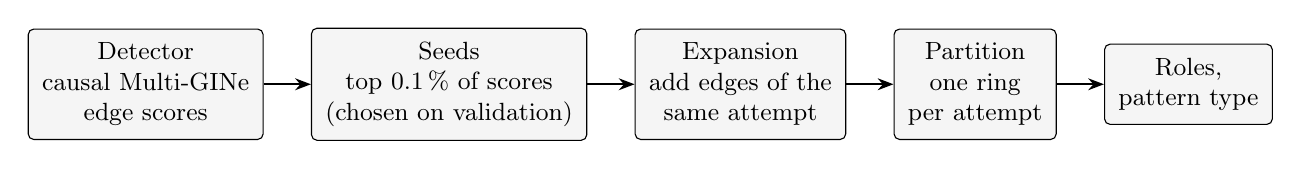
\begin{tikzpicture}[
  node distance=5mm and 6mm,
  stage/.style={draw, rounded corners=2pt, align=center, font=\small,
                minimum height=9mm, inner sep=5pt, fill=gray!8},
  arr/.style={-{Stealth[length=2mm]}, thick}
]
\node[stage] (l1) {Detector\\causal Multi-GINe\\edge scores};
\node[stage, right=of l1] (l2) {Seeds\\top 0.1\,\% of scores\\(chosen on validation)};
\node[stage, right=of l2] (l3a) {Expansion\\add edges of the\\same attempt};
\node[stage, right=of l3a] (l3b) {Partition\\one ring\\per attempt};
\node[stage, right=of l3b] (l3c) {Roles,\\pattern type};
\draw[arr] (l1) -- (l2);
\draw[arr] (l2) -- (l3a);
\draw[arr] (l3a) -- (l3b);
\draw[arr] (l3b) -- (l3c);
\end{tikzpicture}
\caption{The reference pipeline. ``B0'' denotes seeds grouped by connected components with no
further stage.}
% source: docs/report.md §3.2 (architecture, redrawn)
\label{fig:pipeline}
\end{figure}

\paragraph{Detector.}
A Multi-GINe edge classifier~\citep{egressy2024} with port numbering, time deltas, reverse
message passing, ego identifiers and subgraph-pattern edge features~\citep{blanusa2024},
trained with 5 seeds under batch-causal neighbour sampling (look-ahead within a batch of up to
1{,}800\,s; Section~\ref{sec:data}).
% source: docs/report.md §5.2
Causality matters here: a forward-looking variant of one cycle feature read edges after the
scored transaction and inflated its lift over the base rate by 12--16$\times$; made trailing,
the lift falls to 1.0--4.0$\times$ with primary-window edge F1 unchanged (0.495 vs.\ 0.494).
% source: docs/FINDINGS.md (C4)

\paragraph{Seeds.}
Seeds are the top $k^{*}=0.1\,\%$ of raw scores. The budget is fixed in advance for every detector
and seed; \texttt{min\_size} is chosen on validation ring-F1 (it is 3 throughout). As a sensitivity
analysis we also let validation choose $k^{*}$: it picks 0.1\,\% for every seed of Multi-GINe, but
0.05\,\% for two of five MEGA-GNN seeds, which lowers MEGA-GNN's full-pipeline ring-F1 from 0.602 to
0.510 (Table~\ref{tab:detector-swap}).
% source: configs/threshold_rule_k010.yaml; results/tables/r4_partition.csv (chosen_cells); results/tables/r6_detector_swap_sb2048_valpicked.csv (mega full 0.5098; seeds 4, 5 seed_frac_pct 0.05)

\paragraph{Expansion.}
A member edge below the seed cut --- a \emph{quiet member} --- never enters a baseline ring.
Expansion considers candidates that share an endpoint with an included edge within a
validation-chosen $\Delta t$ (up to two hops, capped at the 500 events nearest in time per
account to neutralise hub accounts).
% source: docs/EXPANSION.md §6.1
A LightGBM policy~\citep{ke2017} scores each candidate on 70 causal features: timing, money
conservation at the shared account, direction, reach to other seeds, trailing account state,
embedding similarity, detector-score quantile and trailing pattern counts.
% source: docs/EXPANSION.md §6.2
Its training data is cross-scored --- fold models trained on other days score each held-out
day --- so the policy never learns from in-sample detector scores; rows from day 0 are
dropped.
% source: docs/EXPANSION.md §6.3
The folds hold out days, not rings; Section~\ref{sec:limitations} reports the resulting leak
and its bound. We compare the policy with two rules: \emph{B1}, add every candidate sharing an
endpoint within $\Delta t$; and \emph{B1b}, the same with the candidate's score quantile above
0.99.
% source: docs/FINDINGS.md (B1)

\paragraph{Partition, roles and typing.}
A LightGBM affinity model scores pairs of ring edges that share an account, and
average-linkage clustering with a validation-chosen cut splits merged components. Each ring
then receives account roles from money-conservation rules and one of the eight pattern types
from a classifier over role counts, depth, cycle presence and size.
% source: docs/report.md §5.2

The project also delivers a deterministic explanation layer and a multi-bank analyst platform
on top of these rings. Neither is evaluated as a research claim here; both are summarised in
Appendix~\ref{app:platform}.
        % 5 Reference pipeline
\section{Results with the reference pipeline}
\label{sec:results}

\subsection{Expansion recovers quiet members, and a two-line rule matches it}
\label{sec:results-expansion}

The detector reaches primary-window edge F1 $0.495 \pm 0.027$ and ROC-AUC 0.965.
% source: results/tables/r1_edge_metrics.csv (label=causal); docs/FINDINGS.md (A4)
Table~\ref{tab:ring-methods} gives the ring-level picture; Section~\ref{sec:results-baselines}
discusses the baselines in its upper block.

% Source: results/tables/r9_ring_ci.csv (rows b0, b1, b1b, proposed, average; window=primary) and
%         results/tables/v45_posthoc_ring_ci.csv (baselines and ring-folded rows; produced by
%         evaluation/r9_style_ci.py, which runs evaluation/step9_tables.py unmodified, so every
%         interval in this table is the same ring bootstrap: ring_stats.bootstrap_over_rings).
% Quiet-member recall is the point estimate from r9_quiet_members.csv / v45_posthoc_quiet_members.csv
% (FINDINGS convention, 2026-11-12), not the bootstrap mean in r9_ring_ci.csv.
\begin{table}[t]
\centering
\caption{Ring recovery on the primary window (174 truth rings, 5 seeds or runs,
in-window members, Jaccard $\ge 0.5$). Brackets: 95\,\% bootstrap intervals over truth rings,
seeds averaged inside each resample. Rows marked $^{*}$ use expansion-policy inputs folded by
ring (leak-free); the rows directly above them are the same methods with day-folded inputs, as
first reported. Rows marked $^{\S}$ are post hoc.}
\label{tab:ring-methods}
\small
\begin{tabular}{lccccc}
\toprule
Method & Ring prec. & Ring rec. & Ring F1 [95\,\% CI] & Member cov. & Quiet-member rec. \\
\midrule
CSGM~\citep{tian2025}$^{\dagger\S}$ & 0.321 & 0.048 & \ci{0.083}{0.047}{0.123} & 0.898 & --- \\ % source: v45_posthoc_ring_ci.csv (csgm, primary: 0.3208 / 0.0483 / 0.0834 [0.0474, 0.1227] / 0.8982)
Louvain, resolution 0.5$^{\S}$ & 0.795 & 0.382 & \ci{0.515}{0.428}{0.600} & 0.853 & 0.001 \\ % source: v45_posthoc_ring_ci.csv (louvain_r0.5); quiet v45_posthoc_quiet_members.csv (0.0013)
Louvain, resolution 1$^{\S}$ & 0.748 & 0.358 & \ci{0.483}{0.397}{0.563} & 0.834 & 0.009 \\ % source: v45_posthoc_ring_ci.csv (louvain_r1); quiet 0.0085
Louvain, resolution 2$^{\S}$ & 0.419 & 0.062 & \ci{0.107}{0.070}{0.148} & 0.655 & 0.002 \\ % source: v45_posthoc_ring_ci.csv (louvain_r2); quiet 0.0021
Label propagation$^{\S}$ & 0.785 & 0.377 & \ci{0.509}{0.421}{0.593} & 0.847 & 0.001 \\ % source: v45_posthoc_ring_ci.csv (lpa); quiet 0.0013
\midrule
Seeds + connected components & 0.814 & 0.384 & \ci{0.521}{0.429}{0.607} & 0.866 & 0.005 \\ % source: r9_ring_ci.csv (b0,primary)
Fixed expansion rule    & 0.171 & 0.162 & \ci{0.162}{0.118}{0.213} & 0.970 & 0.118 \\ % source: r9_ring_ci.csv (b1,primary); quiet: r9_quiet_members.csv (b1,primary,ALL = 0.1183)
Rule + score quantile  & 0.702 & 0.463 & \ci{0.555}{0.470}{0.632} & 0.943 & 0.223 \\ % source: r9_ring_ci.csv (b1b,primary); quiet: r9_quiet_members.csv (b1b,primary,ALL = 0.2229)
Learned expansion & 0.838 & 0.446 & \ci{0.582}{0.490}{0.668} & 0.942 & 0.209 \\ % source: r9_ring_ci.csv (proposed,primary); quiet: r9_quiet_members.csv (proposed,primary,ALL = 0.2092)
\quad ring-folded inputs$^{*\S}$ & 0.784 & 0.468 & \ci{0.585}{0.498}{0.670} & 0.960 & 0.251 \\ % source: v45_posthoc_ring_ci.csv (proposed_ringfold: 0.7835 / 0.4678 / 0.5848 [0.4980, 0.6699] / 0.9603); quiet 0.2510
\quad community step instead of components$^{\S}$ & 0.781 & 0.431 & \ci{0.555}{0.466}{0.641} & 0.897 & --- \\ % source: v45_posthoc_ring_ci.csv (lpa_on_expansion: 0.7806 / 0.4310 / 0.5550 [0.4663, 0.6408] / 0.8974)
\textbf{Full (expansion + partition)} & \textbf{0.818} & \textbf{0.461} & \textbf{\ci{0.589}{0.502}{0.675}} & \textbf{0.944} & \textbf{0.203} \\ % source: r4_partition.csv (average) / r9_ring_ci.csv (average,primary)
\quad ring-folded inputs$^{*\S}$ & 0.760 & 0.483 & \ci{0.589}{0.503}{0.672} & 0.960 & 0.243 \\ % source: v45_posthoc_ring_ci.csv (full_ringfold: 0.7597 / 0.4828 / 0.5893 [0.5034, 0.6722] / 0.9604); quiet 0.2425
\bottomrule
\multicolumn{6}{l}{\footnotesize $^{\dagger}$ External baseline, no detector; five runs over random two-institution splits of the accounts.}\\
\multicolumn{6}{l}{\footnotesize Community rows: the method run on the graph of the top-$k$\,\% flagged edges, $k$ chosen on validation per seed.}\\
\multicolumn{6}{l}{\footnotesize ``Community step instead of components'': label propagation on the learned expansion's subgraph, nothing tuned.}\\
\end{tabular}
\end{table}


Expansion from seeds recovers ring members the detector never fires on. With leak-free policy
inputs (Section~\ref{sec:limitations}), quiet-member recall rises from \ci{0.0052}{0.000}{0.015}
with seeds alone to \ci{0.251}{0.179}{0.344} with the learned policy, significant both on quiet
accounts per ring ($+0.432$ [$+0.301$, $+0.590$]) and on whole-ring matching ($+0.084$ [$+0.053$,
$+0.117$]), both $p_{\mathrm{Holm}}=0.0004$.
% source: results/notes/p2_ringfold.md (post hoc table); results/tables/v39_ringfold_quiet_members.csv; v39_ringfold_significance.csv (proposed_ringfold_vs_b0)
With the day-folded inputs we first reported and pre-registered, the recall was
\ci{0.2092}{0.142}{0.290}, with paired differences of $+0.359$ [$+0.236$, $+0.510$] and $+0.062$
[$+0.036$, $+0.092$], both $p_{\mathrm{Holm}}=0.0005$.
% source: results/tables/r9_quiet_members.csv (b0/proposed, primary, ALL); CIs r9_ring_ci.csv; r9_significance.csv (proposed_vs_b0)
It is the only one of the five pre-registered matched-ring comparisons to survive correction
(Table~\ref{tab:significance}), and the result is stable across seed budgets: expansion
recovers 14--24\,\% of quiet members at every budget we tried
(Table~\ref{tab:robustness}, appendix).
% source: docs/FINDINGS.md (section E)

% Source: results/tables/r9_significance.csv (all five pre-registered comparisons)
\begin{table}[t]
\centering
\caption{The five pre-registered comparisons: paired sign-flip permutation tests on per-ring
matched indicators (10{,}000 permutations), Holm-corrected. $\Delta$ is the per-ring matched
rate; the quiet-member column is the per-ring quiet-accounts delta where the family
pre-registered it. The test is blind to precision (Section~\ref{sec:data-stats}).}
\label{tab:significance}
\small
\begin{tabular}{llccc}
\toprule
Comparison & Metric & $\Delta$ [95\,\% CI] & $p_{\mathrm{Holm}}$ & Reject at 0.05 \\
\midrule
proposed vs.\ B0  & matched rate & $+0.062$ [$+0.036$, $+0.092$] & $0.0005$ & yes \\ % source: r9_significance.csv (proposed_vs_b0, mean_delta, p_holm)
proposed vs.\ B0  & quiet accounts/ring & $+0.359$ [$+0.236$, $+0.510$] & $0.0005$ & yes \\ % source: r9_significance.csv (proposed_vs_b0, quiet_mean_delta, quiet_p_holm)
proposed vs.\ B1b & matched rate & $-0.017$ [$-0.041$, $+0.005$] & $0.49$ & no \\ % source: r9_significance.csv (proposed_vs_b1b)
proposed vs.\ B1b & quiet accounts/ring & $-0.024$ [$-0.084$, $+0.037$] & $1.00$ & no \\ % source: r9_significance.csv (proposed_vs_b1b, quiet columns)
full vs.\ expansion only & matched rate & $+0.015$ [$-0.002$, $+0.036$] & $0.49$ & no \\ % source: r9_significance.csv (full_vs_b2)
cc+partition vs.\ B0 & matched rate & $+0.018$ [$+0.002$, $+0.039$] & $0.23$ & no \\ % source: r9_significance.csv (cc_partition_vs_b0)
full vs.\ B1b & matched rate & $-0.002$ [$-0.032$, $+0.028$] & $0.94$ & no \\ % source: r9_significance.csv (full_vs_b1b)
\bottomrule
\end{tabular}
\end{table}


\textbf{The learned policy is not what produces this recovery.} The rule B1b reaches
\ci{0.2229}{0.163}{0.299} quiet recall, indistinguishable from the policy on quiet accounts
($-0.024$ [$-0.084$, $+0.037$], $p_{\mathrm{Holm}}=1.00$) and on whole-ring matching
($p_{\mathrm{Holm}}=0.49$).
% source: docs/FINDINGS.md (B1, B2); r9_significance.csv (proposed_vs_b1b)
We ran this comparison on purpose, against our own method.

What the policy buys is the purity of what it adds. With leak-free policy inputs (cross-scores
folded by ring; Section~\ref{sec:limitations}) its added-member precision is 0.819 against the
rule's 0.518, a paired difference of $+0.301$ [$+0.235$, $+0.366$]; with the day-folded inputs we
first reported, the same comparison gave 0.926 and $+0.408$ [$+0.342$, $+0.479$],
$p_{\mathrm{Holm}}=0.0008$ (Figure~\ref{fig:quiet-precision}, Table~\ref{tab:precision-paired}).
The leak-free comparison was run after the main results and is exploratory.
% source: results/tables/v39_ringfold_precision_paired.csv (proposed_ringfold_vs_b1b, added_member_precision: 0.8190 vs 0.5179, +0.3011 [+0.2349, +0.3657]); v35_precision_paired.csv (proposed_vs_b1b); paper/PREREG_AMENDMENT_2026-11-14.md §3
The matched-ring test cannot see this difference, which is why we test it with the
precision-aware paired bootstrap of Section~\ref{sec:data-stats}. The same test resolves the
gap between the pipeline on Multi-GINe scores and on GFP-XGBoost scores
($+0.139$ ring-F1 [$+0.083$, $+0.196$], $p_{\mathrm{Holm}}=0.0008$), which the matched-ring
test had scored at $p=0.807$: the weaker detector's pipeline matches about as many rings but
adds 2{,}419 edges at 26\,\% precision (day-folded inputs). The policy's ring-F1 gain over the
rule ($+0.027$) does not survive correction ($p_{\mathrm{Holm}}=0.093$); with leak-free inputs
it is $+0.030$ [$+0.010$, $+0.050$], outside the registered family.
% source: results/tables/v35_precision_paired.csv; docs/deep-analysis.md §2; v39_ringfold_precision_paired.csv (proposed_ringfold_vs_b1b, ring_f1: +0.0295 [+0.0101, +0.0501])

\begin{figure}[t]
\centering
\includegraphics[width=0.55\textwidth]{r9_quiet_vs_precision.png}
\caption{Quiet-member recall against added-member precision (day-folded policy inputs, as first
reported; with leak-free inputs the policy's added-member precision is 0.819). The rule and the
policy recover similar shares of quiet members; they differ in how many wrong edges they add.}
% source: results/figures/r9_quiet_vs_precision.png (repository figure)
\label{fig:quiet-precision}
\end{figure}

% Source: results/tables/v35_precision_paired.csv (all eight rows)
\begin{table}[t]
\centering
\caption{Precision-aware paired bootstrap (392 ring-level units, 10{,}000 paired draws, Holm
across four comparisons per metric; primary window, 5 seeds). $p = 0.0002$ raw is the
resolution floor: no draw crossed zero.}
\label{tab:precision-paired}
\small
\begin{tabular}{llccc}
\toprule
Comparison (A vs.\ B) & Metric & $\Delta$ (A $-$ B) [95\,\% CI] & $p_{\mathrm{Holm}}$ & Reject \\
\midrule
proposed vs.\ B1b & added-member prec. & $+0.408$ [$+0.342$, $+0.479$] & $0.0008$ & yes \\ % source: v35_precision_paired.csv (proposed_vs_b1b, added_member_precision)
full vs.\ B1b & added-member prec. & $+0.408$ [$+0.341$, $+0.479$] & $0.0008$ & yes \\ % source: v35_precision_paired.csv (full_vs_b1b, added_member_precision)
GINe full vs.\ GFP-XGB full & added-member prec. & $+0.666$ [$+0.557$, $+0.752$] & $0.0008$ & yes \\ % source: v35_precision_paired.csv (gine_full_vs_gfpxgb_full, added_member_precision)
MEGA full vs.\ GINe full & added-member prec. & $+0.006$ [$-0.042$, $+0.053$] & $0.771$ & no \\ % source: v35_precision_paired.csv (mega_full_vs_gine_full, added_member_precision)
\midrule
proposed vs.\ B1b & ring F1 & $+0.027$ [$+0.001$, $+0.052$] & $0.093$ & no \\ % source: v35_precision_paired.csv (proposed_vs_b1b, ring_f1)
full vs.\ B1b & ring F1 & $+0.034$ [$+0.004$, $+0.065$] & $0.093$ & no \\ % source: v35_precision_paired.csv (full_vs_b1b, ring_f1)
GINe full vs.\ GFP-XGB full & ring F1 & $+0.139$ [$+0.083$, $+0.196$] & $0.0008$ & yes \\ % source: v35_precision_paired.csv (gine_full_vs_gfpxgb_full, ring_f1)
MEGA full vs.\ GINe full & ring F1 & $+0.018$ [$-0.016$, $+0.053$] & $0.303$ & no \\ % source: v35_precision_paired.csv (mega_full_vs_gine_full, ring_f1)
\midrule
\multicolumn{5}{l}{\emph{Leak-free (ring-folded) policy inputs, post hoc; raw $p$, no family correction}}\\
proposed vs.\ B1b & added-member prec. & $+0.301$ [$+0.235$, $+0.366$] & $0.0002^{\P}$ & --- \\ % source: v39_ringfold_precision_paired.csv (proposed_ringfold_vs_b1b, added_member_precision; p_raw 0.0002)
full vs.\ B1b & added-member prec. & $+0.300$ [$+0.233$, $+0.364$] & $0.0002^{\P}$ & --- \\ % source: v45_ringfold_full_precision_paired.csv (full_ringfold_vs_b1b, added_member_precision; p_raw 0.0002)
ring-folded vs.\ day-folded full & added-member prec. & $-0.108$ [$-0.167$, $-0.060$] & $0.0002^{\P}$ & --- \\ % source: v45_ringfold_full_precision_paired.csv (full_ringfold_vs_full)
proposed vs.\ B1b & ring F1 & $+0.030$ [$+0.010$, $+0.050$] & $0.003^{\P}$ & --- \\ % source: v39_ringfold_precision_paired.csv (proposed_ringfold_vs_b1b, ring_f1; p_raw 0.0034)
full vs.\ B1b & ring F1 & $+0.034$ [$+0.008$, $+0.061$] & $0.008^{\P}$ & --- \\ % source: v45_ringfold_full_precision_paired.csv (full_ringfold_vs_b1b, ring_f1; p_raw 0.0082)
ring-folded vs.\ day-folded full & ring F1 & $-0.000$ [$-0.017$, $+0.019$] & $0.96^{\P}$ & --- \\ % source: v45_ringfold_full_precision_paired.csv (full_ringfold_vs_full, ring_f1: -0.0002 [-0.0170, +0.0185], p_raw 0.9617)
\bottomrule
\multicolumn{5}{l}{\footnotesize $^{\P}$ Raw $p$. These draws use 273 units (174 truth rings and 99 off-ring clusters over the methods in that run).}\\
\end{tabular}
\end{table}


\subsection{Community detection is not a stronger baseline than components}
\label{sec:results-baselines}

Replacing connected components with community detection on the same flagged-edge graph does
not help (Table~\ref{tab:ring-methods}, upper block; edge weight is the larger detector score
between two accounts, and the seed fraction is chosen on validation per seed). The best
community method by validation ring-F1, Louvain at resolution 0.5, reaches 0.515 on test,
against 0.521 for seeds and connected components ($-0.006$ [$-0.014$, $+0.000$],
$p_{\mathrm{Holm}}=0.072$) and 0.589 for the full pipeline ($-0.074$ [$-0.118$, $-0.035$],
$p_{\mathrm{Holm}}=0.0004$). Higher resolutions split rings apart (Louvain at resolution 2:
0.107). On the learned policy's expanded subgraph, label propagation in place of components
gives 0.555, below both components (0.582) and the average-linkage partition (0.589). CSGM,
collaborative scatter-gather mining~\citep{tian2025}, is designed for one pattern family and
uses no detector; over five random two-institution splits it reaches 0.083, with ring recall
0.048 over all eight pattern types. These comparisons were added after the main results.
% source: results/tables/v40_external_baselines.json (bar_B: louvain_r0.5 best by val; compare vs b0 / full, paired unit bootstrap 10,000 draws, Holm over two); v45_posthoc_ring_ci.csv (test_visible rows); results/notes/p3_baselines.md

\subsection{Partition: not significant at 174 rings, resolved at 2{,}187}
\label{sec:results-partition}

On HI-Small the partition stage is not significant ($+0.015$ matched rate
[$-0.002$, $+0.036$], $p_{\mathrm{Holm}}=0.49$), nor is partitioning without expansion
($p_{\mathrm{Holm}}=0.23$). On HI-Medium, with 2{,}187 rings, an effect of the same size is
resolved: $+0.015$ [$+0.010$, $+0.020$], $p_{\mathrm{Holm}}=0.0003$
(Section~\ref{sec:results-hm}).
% source: results/tables/v3_closeout_p3.csv (global, full vs b2: mean_delta 0.01486, lo 0.00983, hi 0.01989, p_holm 0.0003)
Its pre-registered hypothesis --- that partitioning would allow a
looser seed budget --- was rejected: validation ring-F1 falls from 0.593 to 0.194 as the seed
fraction grows from 0.10\,\% to 0.50\,\%. A Louvain partition of the same expanded subgraph
leaves ring-F1 unchanged at 0.582.
% source: r9_significance.csv (full_vs_b2, cc_partition_vs_b0); docs/FINDINGS.md (B3, B4); results/tables/r4_partition.csv (b4)
On MEGA-GNN scores, where merged rings are commoner, the gain is the same size ($+0.017$)
and its interval excludes zero ($p_{\mathrm{Holm}} \approx 0.011$): over-merged rings fall
from 9.8 to 8.2 per seed there and stay at 5.2 on ours. The stage removes over-merges only
where they exist, and pays for recall with precision on both detectors.
% source: docs/FINDINGS.md (B3)
Its apparent benefit also depends on two evaluation choices: the recall gain is $+0.024$ at
Jaccard 0.3, $+0.015$ at 0.5 and $+0.001$ at 0.7, and it reverses when only connected pieces
of three or more accounts are scored (Section~\ref{sec:findings-scope}), on both releases.
On HI-Small we do not claim the partition step beyond neutral. Typing, held-out pattern types and time-to-detection are
reported in Appendix~\ref{app:tables}.
% source: docs/FINDINGS.md (B3; dated note, component-level scope)

\subsection{The same pipeline on a larger release}
\label{sec:results-hm}

On HI-Medium the pipeline recovers far less: full-pipeline ring recall is
\ci{0.187}{0.174}{0.200} against HI-Small's 0.461 (Table~\ref{tab:hm-closeout}), 28.7\,\% of rings
are untouched by any seed or expanded edge, and 8.6\,\% are recovered only in part. Its
detector did not meet the adequacy bar fixed before the run, and only two of its three seeds
are usable (Section~\ref{sec:findings-saturation}), so these are not method results on a par
with HI-Small's.
% source: results/tables/v3_closeout_p1.csv (global,full,ring_recall); v3_closeout_verdicts.json (P2_global shares: b_untouched 0.2867, c_under_covered 0.0855); docs/deep-analysis.md §7
Ring-F1 also falls with distance from training: with seeds allocated per day, seed 1 scores
0.408 on test days 6--7 and 0.066 on days 14--15.
% source: results/tables/v3_closeout_blocks.csv (seed 1, per_day, full, ring_f1: block6-7 0.4078, block14-15 0.0656)
What the larger release does provide is power. The partition gain that is not significant on
HI-Small is resolved here at the same size, and the learned policy matches more rings than the
rule ($+0.047$ [$+0.037$, $+0.057$], $p_{\mathrm{Holm}}=0.0003$), where on HI-Small the two were
indistinguishable.
% source: results/tables/v3_closeout_p3.csv (global: full vs b2 +0.0149 [+0.0098, +0.0199]; policy vs b1b +0.0471 [+0.0373, +0.0572]; p_holm 0.0003)

% Source: results/tables/v3_closeout_p1.csv (point / lo / hi), v3_closeout_p3.csv. Intervals: ring bootstrap
% (evaluation/ring_stats.py::bootstrap_over_rings, 1,000 resamples), the same procedure as the HI-Small headline.
\begin{table}[t]
\centering
\caption{Ring recovery on HI-Medium (2{,}187 in-scope rings, test days 6--14, two detector seeds,
in-window members, Jaccard $\ge 0.5$). Brackets: 95\,\% bootstrap intervals over rings.$^{\ddagger}$}
\label{tab:hm-closeout}
\small
\begin{tabular}{llccc}
\toprule
Seed allocation & Method & Ring rec. & Rec. (rings $\ge$3) & Ring F1 \
\midrule
global  & learned expansion     & \ci{0.172}{0.159}{0.185} & \ci{0.243}{0.227}{0.260} & \ci{0.180}{0.166}{0.194} \ % source: v3_closeout_p1.csv (global,proposed)
global  & expansion + partition & \ci{0.187}{0.174}{0.200} & \ci{0.264}{0.246}{0.280} & \ci{0.182}{0.169}{0.195} \ % source: v3_closeout_p1.csv (global,full)
per day & learned expansion     & \ci{0.222}{0.207}{0.238} & \ci{0.315}{0.296}{0.336} & \ci{0.233}{0.217}{0.249} \ % source: v3_closeout_p1.csv (per_day,proposed)
per day & expansion + partition & \ci{0.242}{0.226}{0.257} & \ci{0.340}{0.321}{0.360} & \ci{0.234}{0.219}{0.249} \ % source: v3_closeout_p1.csv (per_day,full)
\bottomrule
\multicolumn{5}{l}{\footnotesize $^{\ddagger}$ Detector seeds 1--2 only (seed 3's scores saturate); the detector did not meet its}\
\multicolumn{5}{l}{\footnotesize pre-registered adequacy bar. Not pooled with HI-Small.}\
\end{tabular}
\end{table}


\subsection{Edge F1 is not a proxy for ring recovery}
\label{sec:results-swap}

We re-ran the ring layer on other detectors at the same fixed 0.1\,\% seed budget, re-choosing
every other downstream parameter on validation per detector and seed (Figure~\ref{fig:edge-ring}, Table~\ref{tab:detector-swap}).
Our MEGA-GNN reproduction reaches $0.6856 \pm 0.0447$ test edge F1, against the
$0.7083 \pm 0.0218$ its authors report for the same configuration; the gap is attributable to
batch-causal sampling (Section~\ref{sec:data}), which their setup does not use\footnote{All MEGA-GNN scores in this paper are produced with a scoring batch of 2048 transactions. The released models were originally scored at 8192, which gives test edge F1 $0.6893 \pm 0.0396$ against $0.6856 \pm 0.0447$ at 2048; per seed, 2048 minus 8192 is $-0.0126$, $-0.0029$, $-0.0013$, $+0.0049$ and $-0.0069$. The causal neighbour sampler cuts batches by size or by 30 minutes of seed time, whichever comes first, so a larger scoring batch lets a transaction see later transactions of the same batch (median look-ahead 180\,s at 2048, 600\,s at 8192). The validation-to-test gap per seed is in Table~\ref{tab:val-test-gap}.}.
% source: results/notes/p7_genagg.md (batch-2048 per-seed table, look-ahead); results/notes/p7_batch_span.json
% Pass 2 (2026-11-16): Table detector_swap and the edge-F1 sentence above now use batch 2048 (r6_detector_swap_sb2048.csv).
% TODO pass 2, still at 8192 and needing recomputation at 2048 before they change: "9.4 points" (2048 gives 0.6856 - 0.5957 = 9.0;
%   also abstract, introduction, conclusion, figure caption); B0 "0.5208 vs 0.5213" (2048: 0.5179); seed-set Jaccard 0.415 and
%   "128.8 and 129.6" rings reached (2048 rings_touched 127.4; seed Jaccard not yet recomputed); fig_edge_vs_ring; scope_sensitivity
%   and component_scope MEGA rows. See results/notes/p5_required_changes.md.
% source: docs/paper/generalisation.md §1

\begin{figure}[t]
\centering
\includegraphics[width=0.62\textwidth]{fig_edge_vs_ring.png}
\caption{Edge F1 against ring F1 for three detectors. From Multi-GINe to MEGA-GNN, 9.4 points
of edge F1 buy no change in ring F1 at the baseline operating point; below Multi-GINe, ring
F1 falls with edge F1.}
% source: results/tables/r6_detector_swap.csv; figure built by paper_draft/make_figs.py
\label{fig:edge-ring}
\end{figure}

% Source: results/tables/r6_detector_swap.csv (GFP-XGBoost, Multi-GINe); results/tables/r6_detector_swap_sb2048.csv (MEGA-GNN rows, scoring batch 2048)
\begin{table}[t]
\centering
\caption{The same ring layer on several detectors at the fixed 0.1\,\% seed budget, every other
downstream parameter re-chosen on validation per detector per seed. With the budget chosen on
validation instead (sensitivity), MEGA-GNN's ring F1 falls to 0.414 (B0) and 0.510 (full); the
Multi-GINe and GFP-XGBoost rows are unchanged. Edge F1 is on the whole test split (mean $\pm$
std over 5 seeds); ring numbers are on the primary window with bootstrap CIs. MEGA-GNN is scored with a batch of 2048 transactions (Section~\ref{sec:results-swap}). Added-member precision here was measured with day-folded expansion-policy inputs; with leak-free (ring-folded) inputs the reference full pipeline's value is 0.817 (Table~\ref{tab:precision-paired}).}
% source (leak-free value): results/tables/v45_ringfold_full_precision_paired.csv (full_ringfold, added_member_precision 0.8174)
\label{tab:detector-swap}
\small
\begin{tabular}{lccccc}
\toprule
Detector & Edge F1 & Ring F1, B0 & Ring F1, full & Quiet rec., full & Added prec., full \\
\midrule
GFP-XGBoost & $0.500 \pm 0.006$ & \ci{0.343}{0.259}{0.426} & \ci{0.451}{0.375}{0.526} & 0.267 & 0.260 \\ % source: r6_detector_swap.csv (gfpxgb rows)
Multi-GINe (shipped) & $0.596 \pm 0.071$ & \ci{0.521}{0.429}{0.607} & \ci{0.589}{0.502}{0.675} & 0.203 & 0.926 \\ % source: r6_detector_swap.csv (gine_causal rows)
MEGA-GNN & $0.686 \pm 0.045$ & \ci{0.518}{0.429}{0.604} & \ci{0.602}{0.517}{0.683} & 0.234 & 0.915 \\ % source: r6_detector_swap_sb2048.csv (mega b0 / full rows, scoring batch 2048)
MEGA-GNN, no embeddings & $0.686 \pm 0.045$ & -- & \ci{0.578}{0.493}{0.659} & 0.200 & 0.787 \\ % source: r6_detector_swap_sb2048.csv (mega_noembed full row)
MEGA-GenAgg & \textit{[TBD]} & \textit{[TBD]} & \textit{[TBD]} & \textit{[TBD]} & \textit{[TBD]} \\ % TODO pass 2: GenAgg placeholder; fill from the five-seed rows once seed 5 is scored
\bottomrule
\end{tabular}
\end{table}


MEGA-GNN outscores Multi-GINe by 9.4 points of edge F1 and produces the same baseline rings
(ring-F1 0.5208 vs.\ 0.5213) at the fixed budget. When validation chooses the budget instead,
two MEGA-GNN seeds pick 0.05\,\% and its rings fall behind (Section~\ref{sec:method}).
% source: results/tables/r6_detector_swap.csv; docs/FINDINGS.md (C6)
This is not the detectors agreeing. Their seed sets overlap at Jaccard 0.415, yet they reach
128.8 and 129.6 of the 174 truth rings. What binds at this operating point is how many rings a
0.1\,\% quantile can reach, not the ranking that fills it. The relation is a ceiling, not
independence: the weaker GFP-XGBoost, 9.6 edge points below, loses 17.7 ring points.
% source: docs/FINDINGS.md (C6)
The claim is conditional on this budget, these detectors and this dataset; a detector
stronger than MEGA-GNN was not tested.

\paragraph{Can the budget be spent better?}
Each GNN detector touches about 74\,\% of truth rings and their touched sets overlap at
71.5\,\%, so their union reaches 150.8 of 174 --- but that is two full budgets. At the same
budget, a best-rank ensemble of the two reaches 133.6, about a fifth of the gap, because 484
of the 864 selected edges are in both detectors' top 0.1\,\%. A per-account budget reaches
fewer (116.2). At an equal budget neither reallocation changes baseline ring-F1 beyond seed
noise (0.521 / 0.515 / 0.519), and under the full pipeline the ensemble's gain
($+0.021 \pm 0.038$) is inside seed spread.
% source: docs/FINDINGS.md (C7, B14 with its dated correction); results/tables/v37_realloc_full.csv

\paragraph{The effective test budget is about half the nominal one.}
Because the quantile is taken over the whole test split, only 463 of 864 seeds land in the
primary window (Section~\ref{sec:findings-tail}). Spending the full budget inside the window
reaches 148.2 rings instead of 129.6 and leaves 28.0 rings untouched instead of 33.2. But
added-member precision (day-folded policy inputs) falls from 0.926 to 0.700, below a 0.85
bound fixed in advance, and
ring-F1 falls from 0.589 to 0.546, on every seed (Table~\ref{tab:window-budget}). The extra
seeds are weaker, and expanding from them costs more rings than the new reach gains. The
budget binds, then, at about 463 in-window seeds, and the reported ring-F1 is not depressed by
the budget lost to the tail. This is a sensitivity analysis on a window examined many times,
and downstream parameters were deliberately not re-tuned.
% source: results/tables/v34_window_budget.json; docs/deep-analysis.md §1

% Source: results/tables/v34_window_budget.json (summary), as tabulated in docs/deep-analysis.md §1
\begin{table}[t]
\centering
\caption{Window-matched seed budget (mean $\pm$ SD over 5 seeds, primary window, 174 truth
rings). Only the seed mask changes; every downstream cell is the shipped, validation-chosen
one. A sensitivity row, not a re-selection: the shipped rule stays the best on ring-F1. Added-member precision here was measured with day-folded expansion-policy inputs; with leak-free (ring-folded) inputs the reference full pipeline's value is 0.817 (Table~\ref{tab:precision-paired}).}
\label{tab:window-budget}
\small
\begin{tabular}{lccc}
\toprule
 & Global (shipped) & In-window quantile & Per-day quantile \\
\midrule
Seeds in window & $463.0 \pm 84.2$ (of 864) & 863 & 864 \\ % source: v34_window_budget.json (seeds_in_window)
Rings touched & $129.6 \pm 4.8$ & $148.2 \pm 6.2$ & $139.8 \pm 7.3$ \\ % source: v34_window_budget.json (rings_touched)
Untouched rings, full & $33.2 \pm 3.6$ & $28.0 \pm 5.5$ & $30.6 \pm 3.8$ \\ % source: v34_window_budget.json (full_b_untouched)
Added-member precision & $0.926 \pm 0.015$ & $0.700 \pm 0.137$ & $0.738 \pm 0.098$ \\ % source: v34_window_budget.json (added_member_precision)
Matched rings, full & $80.2 \pm 5.9$ & $77.6 \pm 5.6$ & $75.8 \pm 5.3$ \\ % source: v34_window_budget.json (full_matched)
Ring F1, full & $0.589 \pm 0.037$ & $0.546 \pm 0.023$ & $0.532 \pm 0.032$ \\ % source: v34_window_budget.json (full_ring_f1)
Ring F1, B0 & $0.521 \pm 0.045$ & $0.503 \pm 0.042$ & $0.485 \pm 0.036$ \\ % source: v34_window_budget.json (b0_ring_f1)
\bottomrule
\end{tabular}
\end{table}


\section{Where ring recovery stops}
\label{sec:results-ceiling}

Figure~\ref{fig:decomposition} accounts for all 174 truth rings. With the full pipeline on the
reference detector, 80.2 are matched per seed, 48.6 have fewer than three visible members and
go unmatched, 33.2 are untouched by any seed or expanded edge, 5.2 are merged with a
neighbour and 6.8 are recovered only in part. Achieved ring recall is
\ci{0.461}{0.393}{0.529}.
% source: docs/FINDINGS.md (B11); results/tables/r6_detector_swap.csv; r9_ring_ci.csv (average, primary, ring_recall)

\begin{figure}[t]
\centering
\includegraphics[width=0.9\textwidth]{fig_ring_decomposition.png}
\caption{What happens to the 174 primary-window truth rings (per seed, full pipeline). A
stronger detector converts untouched rings into matches and into over-merges.}
% source: docs/FINDINGS.md (B11); figure built by paper_draft/make_figs.py
\label{fig:decomposition}
\end{figure}

\paragraph{Small rings are not a hard ceiling.}
60 of the 174 rings have fewer than three visible members, yet the pipeline matches
$11.4 \pm 2.3$ of them per seed, most at Jaccard 1.0, because \texttt{min\_size} applies to
the unrestricted prediction while matching uses the window-restricted one. The share of rings
with three or more visible members (114 of 174) is a reference level, not a bound.
% source: docs/FINDINGS.md (B7, B9, as corrected)

\paragraph{The untouched count belongs to the detector and budget.}
MEGA-GNN at the same budget leaves 24.0 rings untouched instead of 33.2, and 6.4 of the 9.2
newly reached rings become matches. The net matched count rises only from 80.2 to 83.6,
because the stronger detector also merges more rings with their neighbours (5.2 to 8.2).
% source: docs/FINDINGS.md (B8, B11)

\paragraph{Partially recovered rings are clean, short fragments of long patterns.}
In every one of the 34 partially recovered instances the prediction contains no wrong
account, and it holds a median 3 of the ring's 14 members. Thirteen distinct rings produce all
34 instances, half of them STACK.
% source: docs/FINDINGS.md (B12); results/tables/r_under_covered.csv

\paragraph{Most of what is missing is disconnected inside the window.}
For each partially recovered ring we measured the distance from the recovered fragment to the
ring's missing member edges, through the ring itself, inside the primary window. 176 of 216
missing edges (81.5\,\%) lie in a piece with no path to the fragment at all --- all 140 for
STACK, all 24 for BIPARTITE --- and 85.6\,\% were never generated as candidates. The exception
is GATHER-SCATTER, whose 31 missing edges sit one hop away and were declined by the policy; an
oracle admitting exactly those edges completes all 8 instances, about 1.6 rings per seed,
whereas lowering the policy's floor to reach them costs more precision than validation
accepts.
% source: docs/FINDINGS.md (B13, B15); results/tables/r_in_window_connectivity.csv
Widening the window to all ten test days reduces disconnection to 52.3\,\% and removes it for
CYCLE and RANDOM, but STACK stays at 100\,\% (237 of 237): its chains are severed by the
train/validation/test split itself. Traversing the full 18-day graph backwards under the
expansion's own rules reaches none of the 140 missing STACK edges at two or three hops, and a
permutation null reaches none of 216.
% source: docs/FINDINGS.md (B13, B16); results/tables/r_historical_bridge.csv
A supervised-contrastive head~\citep{khosla2020} trained on the frozen detector embeddings to
recognise ring identity does not reconnect the pieces either: same-ring separability across
components rises only from AUC 0.552 to 0.618, against a bar of 0.75 fixed in advance.
% source: docs/deep-analysis.md §10 — registered follow-up; not yet recorded in docs/FINDINGS.md

\paragraph{Observability, counted directly.}
77 of the 174 rings (44\,\%) have no connected in-window piece of three or more accounts. 60
of them are the small rings above; the other 17 have enough visible members, split across
pieces that are each too small, and are scored as ordinary misses. On the 97 rings that do
have a matchable piece, the pipeline recovers 70.6\,\% of the pieces, and STACK recall rises
from 0.036 to 0.493.
% source: docs/FINDINGS.md (dated note, component-level scope); results/tables/v36_component_scope.csv

Taken together, the binding constraint is neither seed allocation nor policy thresholds. It is
how much of a ring is observable and connected inside the evaluation window --- a property of
the split and the scope rule that is easy to mistake for a property of the method.

\subsection{What did not help}
\label{sec:results-negative}
% Pass 2 draft (2026-11-16) from the proposal paragraph in results/notes/m_track.md; descriptive only, no improvement claimed.
We tried five ways of spending the seed budget or reassembling rings after the detector, all at
the fixed 0.1\,\% budget (primary window, test-visible truth, Jaccard 0.5, five seeds). They did not
all use the same reference. Seed fusion and per-account budgets were measured before the leak-free
pipeline existed, against the shipped full pipeline. Account-level seeding was compared with the
shipped full pipeline (0.589). Over-generate-and-verify, motif search and flow-following were
pre-registered against the leak-free full pipeline (0.589 to three decimals; the two pipelines'
ring F1 agree). None raised ring-F1.
\begin{itemize}
\item \emph{Seed fusion and per-account budgets.} A best-rank fusion of two detectors' seeds
gave $+0.021 \pm 0.038$ under the full pipeline, inside seed spread; spreading the budget per
account reached fewer rings and lowered ring-F1.
% source: docs/FINDINGS.md (B14); results/tables/v37_realloc_full.csv
\item \emph{Account-level seeding.} Seeding by account at the same seed count lowered full-pipeline
ring-F1 from \ci{0.589}{0.502}{0.675} to \ci{0.452}{0.377}{0.532} (paired difference $-0.138$
[$-0.184$, $-0.093$]).
% source: results/notes/q_track.md (Q2); results/tables/q_family_holm.csv
\item \emph{Over-generate and verify.} Seeding at twice the budget and filtering with a ring-level
verifier moved ring precision up by $0.098$ [$0.034$, $0.156$] and ring recall down by $0.029$
[$-0.063$, $+0.005$]; the ring-F1 difference, $+0.004$ [$-0.041$, $+0.046$], is
indistinguishable from zero. We report this precision--recall trade as descriptive and secondary.
% source: results/tables/m1_primary.json (other_metrics_paired; primary reading R6 inconclusive, p_Holm 1.00)
\item \emph{Temporal motif search} and \emph{flow-following} from the seeds did not improve on the
seed-only rings. Neither passed its validation gate (best cell 0.569 against 0.585 for the
reference), and their best score-gated cells reproduced the seed-only rings exactly; neither was
run on test.
% source: results/tables/m2_gate.json, m3_gate.json; results/notes/m_track.md (M2, M3)
\end{itemize}
The loss breakdown says why. Of the 174 truth rings in the primary window, 77 have no in-window
piece of three or more accounts (11.4 of them are still matched per seed), 11.0 per seed are
matchable but touched by no seed, 14.4 are recovered too thinly, and merges (1.0) and splits (1.8)
account for little; 68.8 are matched.
% source: results/notes/q_track.md (Q0 table); results/tables/q0_buckets.csv
These counts reconcile with Section~\ref{sec:results-ceiling}: there, the 80.2 matched rings are
$68.8 + 11.4$, and ``untouched'' counts all rings, whereas here it counts only matchable ones.
Reassembly can only rearrange what the seeds already reach, and on this protocol that was not
enough to raise ring-F1.
       % 6 Results; 7 Where recovery stops
\section{Recommendations for reporting ring-level AML results}
\label{sec:recommendations}

Each recommendation below follows from a measurement in this paper.

\begin{enumerate}
\item \textbf{State the scope rule.} Say which accounts count as a ring's members when the
  ring crosses the evaluation window. The choice is worth 0.35--0.38 ring-F1 on HI-Small and
  0.04--0.07 on HI-Medium (Sections~\ref{sec:findings-scope} and~\ref{sec:findings-hm}).
% source: results/tables/r14_scope_sensitivity.csv; results/tables/v41_hm_audit_scope.csv
\item \textbf{State the split and the window, and report the tail separately.} On AMLworld's
  day split, do not average over days 10--17 (Section~\ref{sec:findings-tail}).
\item \textbf{State how a selection budget is allocated across days.} A global quantile can
  give one day most of the budget, and on this split gives the clean window about half
  (Sections~\ref{sec:findings-tail} and~\ref{sec:results-swap}).
\item \textbf{State the tie-handling rule of any quantile cut.} When many scores are tied at
  the cut, ``score $>$ q'' and ``score $\ge$ q'' select very different sets; on one saturated
  HI-Medium detector the strict rule selects no seeds at all
  (Section~\ref{sec:findings-saturation}).
\item \textbf{Sweep the matching threshold.} Report the gain at a stricter threshold wherever
  it is reported at 0.5; a gain that vanishes at 0.7 is fragmentation
  (Section~\ref{sec:results-partition}).
\item \textbf{Resample rings, not edges, and test precision.} Matched-ring tests cannot see
  false rings; pair them with a test that can (Section~\ref{sec:data-stats}).
\item \textbf{Never quote recovered-member recall without the precision of what was added.}
  The weakest detector in our comparison posts the highest quiet-member recall, at 26\,\%
  added-member precision (Table~\ref{tab:detector-swap}).
\item \textbf{Report how many targets are observable.} Count the rings that have a connected,
  matchable piece in the window, and report recall on those beside recall on all
  (Section~\ref{sec:results-ceiling}).
\item \textbf{Do not use edge F1 as evidence of better group recovery.} Run the group-level
  evaluation (Section~\ref{sec:results-swap}).
\item \textbf{Include a rule baseline.} A two-line rule matched our learned component's recall
  (Section~\ref{sec:results-expansion}).
\end{enumerate}

\section{Limitations}
\label{sec:limitations}

\paragraph{One generator family.}
Everything here is AMLworld. The tail and warm-up are reproduced on LI-Small; on HI-Medium the
warm-up, the budget capture, the share of unobservable rings, the threshold dependence of the
partition gain and the direction (not the size) of the scope effect reproduce, from a detector
that missed its adequacy bar and two usable seeds. All three releases come from one simulator;
nothing establishes how the findings carry to other generators or to real transaction data. Method
comparisons rest on 174 truth rings and 5 detector seeds, and only one of five pre-registered
comparisons survives correction at that power.
% source: docs/FINDINGS.md (A6); docs/paper/generalisation.md §3

\paragraph{External baselines.}
We score one external group-level method (CSGM, five random two-institution splits) and two
families of community detection (Louvain at three resolutions, label propagation) under the
protocol. Leiden was planned but not run, and learned sub-network
methods~\citep{chai2023,rico2026} were not run, so we cannot say how the protocol would re-rank
published group-level results.
% source: results/tables/v40_external_baselines.json (runs, notes); results/notes/p3_baselines.md

\paragraph{The edge-versus-ring claim is conditional.}
It is measured at one seed budget, between two GNN detectors about 9 edge-F1 points apart, on
one dataset. Stronger published detectors were not tested.

\paragraph{A ring-level leak in the expansion policy's training data.}
The policy's cross-scored inputs hold out a day per fold, but rings span days, so a fold model
is supervised on some edges of a ring and then scores that ring's held-out-day edges. Between
65.0\,\% and 92.4\,\% of each fold's held-out rings are affected. The measured effect is small
--- the gap in ROC-AUC between affected and unaffected ring edges ranges from $-0.008$ to
$+0.036$ across folds, and unaffected rings are still scored at AUC 0.958--0.996 --- and the
leak touches training inputs only: test scores come from a detector trained on the train
split alone. Removing the affected feature group changes primary-window ring-F1 by 0.008,
which bounds what a leak-free version could change on HI-Small; on HI-Medium the same ablation
moves validation ring-F1 by 0.026 in the opposite direction, so the bound does not transfer
between releases.
% source: docs/FINDINGS.md (B17); results/tables/v33_ring_fold_leakage.csv, v33_leak_inflation.csv, v33_policy_ablations.csv
We re-ran the policy with its inputs folded by ring, so that no fold model sees any edge of a
ring it scores. The registered check on the mean ring-F1 difference passed ($+0.0028$, inside
$\pm 0.008$), but the paired interval, $[-0.0137, +0.0211]$ ($p=0.77$), is too wide to call the
two equivalent, so on ring-F1 the comparison is inconclusive. The leak did inflate precision:
with leak-free inputs, ring precision falls from 0.838 to 0.784 ($-0.055$ [$-0.089$, $-0.027$])
and added-member precision from 0.926 to 0.819, while ring recall rises by 0.022. The full
pipeline behaves the same way: ring-F1 0.589 with either input ($-0.000$ [$-0.017$, $+0.019$]),
added-member precision 0.926 against 0.817. Where this paper reports added-member or ring
precision, the leak-free value is given first. These re-runs were added after the main results
and are exploratory.
% source: docs/deep-analysis.md §8 (verdict) and §15; results/tables/v39_ringfold_report.csv (paired: ring_f1, ring_precision, ring_recall, added_member_precision); v45_ringfold_full_precision_paired.csv (full_ringfold_vs_full); v45_posthoc_ring_ci.csv; paper/PREREG_AMENDMENT_2026-11-14.md

\paragraph{Analyses added after the main results.}
The precision-aware paired test, the window-matched budget, the component-level scope and the
reallocation analysis were run on a test window that had already been examined many times.
Their designs and bars were written down before each was run, but they are sensitivity
analyses, not confirmatory tests. None changes a reported point estimate.
% source: docs/FINDINGS.md (section G preamble); docs/deep-analysis.md (header and caveats)

\paragraph{Published-number comparison.}
The only published figure we compare against is MEGA-GNN's edge F1
(Section~\ref{sec:results-swap}).

\section{Conclusion}
\label{sec:conclusion}

When the unit of evaluation is the laundering attempt, the numbers AMLworld produces are
governed first by choices that papers rarely state and only then by the method. The scope rule
is worth 0.35--0.38 ring-F1. The standard split's tail inflates edge metrics and halves the
effective seed budget in the two days that carry ordinary traffic. And 44\,\% of in-scope
rings cannot be matched as connected objects by any method, because the split and the window
sever them.
% source: docs/FINDINGS.md (C9, C1 and dated notes on the window-matched budget and component-level scope)

Within those limits, a reference pipeline shows what is and is not gained. Growing rings
outward from the detector's strongest edges recovers members the detector never flags (0.5\,\%
to 25\,\% with leak-free policy inputs, at an added-member precision of 0.819; 21\,\% and 0.926 with
the day-folded inputs first reported), and ring-F1 rises from \ci{0.521}{0.429}{0.607} to \ci{0.589}{0.502}{0.675}; on
HI-Small a two-line rule matches that recall, and the learned policy adds purity. Community
detection on the same flagged edges does no better than connected components. Partitioning is
not significant at 174 rings; on HI-Medium, with 2{,}187 rings, an effect of the same size is
resolved. A 9.4-point better edge detector recovers no more rings at the same budget.
% source: results/tables/r9_ring_ci.csv; r4_partition.csv; r9_significance.csv; r6_detector_swap.csv; results/tables/v40_external_baselines.json (bar_B); results/tables/v3_closeout_p3.csv (global, full vs b2)

The practical consequence is for how group-level AML results are reported. A ring-level number
is interpretable only with its scope rule, split, window, budget allocation and matching
threshold attached, and edge F1 is not evidence about it. We release the protocol, the tables
behind every number in this paper, and the code.


% ---- camera-ready only (removed for anonymous review) ----
% \begin{acks}
% % source: CONTRIBUTORS.md
% Ruhani Kumar built the explanation layer and the Elliptic baselines, and found the evaluation
% defect in ring typing that Appendix~\ref{app:corrections} records; Kashish Mittal built the
% multi-tenant platform; Lakshmishree produced the dashboard mockup.
% % source: CONTRIBUTORS.md; docs/FINDINGS.md (typing correction, 2026-10-22)
% \end{acks}
% ----------------------------------------------------------

\bibliographystyle{ACM-Reference-Format}
\bibliography{refs}

% Target: 8 pages including references, no supplementary material. Proposed cuts and moves to the
% released repository (not applied yet): paper/PAGE_BUDGET.md.
\appendix
\section{Reproducibility}
\label{app:repro}

All runs: Intel Xeon W-2295 (18C/36T), 128\,GB RAM, NVIDIA RTX A5000 (24\,GB), Windows 11,
Python 3.12, PyTorch 2.5.1+cu121, PyG 2.8.0.
% source: README.md (Hardware)
Every reported number recomputes from a run's stored metrics; an audit script re-derives 18
headline rows mechanically (18 traceable, 0 mismatched), and a frozen-numbers file pins every
headline to its source with a failing test on change.
% source: README.md; docs/REPRODUCE.md §13 (row 6); results/FROZEN.json

\paragraph{Data integrity.}
Edge identifiers are row positions after a stable sort on timestamps, so a manifest check pins
the inputs:
% source: docs/REPRODUCE.md §0

\begin{center}\small
\begin{tabular}{lll}
\toprule
File & SHA-256 (first 16) & Bytes \\
\midrule
\texttt{HI-Small\_Trans.csv} & \texttt{b19d39f515523373} & 475{,}664{,}283 \\ % source: docs/REPRODUCE.md §0
\texttt{HI-Small\_accounts.csv} & \texttt{786808526e33cfc4} & 34{,}053{,}187 \\ % source: docs/REPRODUCE.md §0
\texttt{HI-Small\_Patterns.txt} & \texttt{2c546b5ce6009e73} & 323{,}844 \\ % source: docs/REPRODUCE.md §0
\texttt{formatted\_transactions.csv} & \texttt{3b9678458eeece7e} & 266{,}605{,}148 \\ % source: docs/REPRODUCE.md §0
\bottomrule
\end{tabular}
\end{center}

\paragraph{End-to-end check.}
With nothing retrained, the data manifest passes, the research test suite passes 258 tests,
and the ring-building command regenerates the released rings byte-identically (108 rings in
62\,s).
% source: docs/REPRODUCE.md §13 (rows 1, 2a, 7)
Measured training times: detector about 15\,h for 5 seeds; cross-scoring about 8\,h; MEGA-GNN
about 18\,h; statistics about 45\,min.
% source: docs/REPRODUCE.md §2, §4, §7, §8

\section{Additional results}
\label{app:tables}

\paragraph{Scope conventions.}
Tables~\ref{tab:scope} and~\ref{tab:component-scope} give the numbers behind
Figure~\ref{fig:scope}.

% Source: results/tables/r14_scope_sensitivity.csv, as summarised in
%         docs/paper/evaluation_protocol.md §9 (same shipped runs re-scored; no model re-run)
\begin{table}[t]
\centering
\caption{The scope convention moves ring-F1 about five times more than the entire method does.
The same shipped runs re-scored under \texttt{full\_membership} (a ring's member set is all its
accounts) against the reported \texttt{test\_visible}; the method ordering survives under both.}
\label{tab:scope}
\small
\begin{tabular}{lccc}
\toprule
Detector / method & \texttt{test\_visible} (reported) & \texttt{full\_membership} & Gap \\
\midrule
GINe B0 & 0.5213 & 0.1437 & $-0.378$ \\ % source: r14_scope_sensitivity.csv (gine_causal b0 rows, ring_f1)
GINe B1b & 0.5553 & 0.2073 & $-0.348$ \\ % source: r14_scope_sensitivity.csv (gine_causal b1b rows)
GINe proposed & 0.5819 & 0.2297 & $-0.352$ \\ % source: r14_scope_sensitivity.csv (gine_causal proposed rows)
GINe full & 0.5894 & 0.2428 & $-0.347$ \\ % source: r14_scope_sensitivity.csv (gine_causal full rows)
MEGA B0 & 0.5208 & 0.1595 & $-0.361$ \\ % source: r14_scope_sensitivity.csv (mega b0 rows)
MEGA full & 0.6074 & 0.2252 & $-0.382$ \\ % source: r14_scope_sensitivity.csv (mega full rows)
\bottomrule
\end{tabular}
\end{table}

% Source: results/tables/v36_component_scope_wci.csv (v36_component_scope.csv re-scored with the
%         weighted ring bootstrap by evaluation/rescore_weighted_intervals.py; point estimates identical)
\begin{table}[t]
\centering
\caption{A third scope convention: each in-window connected piece of a truth ring scored as
its own target (\texttt{component}: 254 targets), or only pieces of $\ge 3$ accounts
(\texttt{component\_ge3}: 108 targets in 97 rings). Ring-F1 with 95\,\% bootstrap CIs over
targets; same shipped runs, nothing re-selected. Denominators differ between conventions, so
the right-hand columns are never headline numbers.}
\label{tab:component-scope}
\small
\begin{tabular}{llccc}
\toprule
Detector & Method & \texttt{test\_visible} & \texttt{component} & \texttt{component\_ge3} \\
\midrule
GINe & B0 & \ci{0.521}{0.429}{0.607} & \ci{0.444}{0.371}{0.514} & \ci{0.673}{0.576}{0.761} \\ % source: v36_component_scope_wci.csv (gine_causal, b0)
GINe & B1b & \ci{0.555}{0.470}{0.632} & \ci{0.488}{0.412}{0.562} & \ci{0.700}{0.628}{0.767} \\ % source: v36_component_scope_wci.csv (gine_causal, b1b)
GINe & proposed & \ci{0.582}{0.490}{0.668} & \ci{0.504}{0.425}{0.572} & \ci{0.766}{0.678}{0.840} \\ % source: v36_component_scope_wci.csv (gine_causal, proposed)
GINe & full & \ci{0.589}{0.502}{0.675} & \ci{0.515}{0.438}{0.583} & \ci{0.740}{0.656}{0.812} \\ % source: v36_component_scope_wci.csv (gine_causal, full)
MEGA & B0 & \ci{0.521}{0.432}{0.609} & \ci{0.441}{0.366}{0.510} & \ci{0.674}{0.588}{0.762} \\ % source: v36_component_scope_wci.csv (mega, b0)
MEGA & proposed & \ci{0.598}{0.506}{0.683} & \ci{0.517}{0.437}{0.583} & \ci{0.777}{0.707}{0.846} \\ % source: v36_component_scope_wci.csv (mega, proposed)
MEGA & full & \ci{0.607}{0.521}{0.688} & \ci{0.530}{0.452}{0.595} & \ci{0.774}{0.709}{0.837} \\ % source: v36_component_scope_wci.csv (mega, full)
\bottomrule
\end{tabular}
\end{table}


\paragraph{Validation-to-test gap.}
Table~\ref{tab:val-test-gap} gives the per-seed edge F1 behind the scoring-batch footnote in
Section~\ref{sec:results-swap}.

% Source: results/notes/p7_val_test_gap.csv (Multi-GINe), results/notes/p7_val_test_gap_sb2048.csv (MEGA-GNN, scoring batch 2048),
% shipped batch-8192 values from results/tables/r6_detector_swap.csv (edge_f1_per_seed)
\begin{table}[t]
\centering
\caption{Validation-to-test edge-F1 gap per seed. The threshold is chosen on validation
(maximum F1 over 400 validation-score quantiles) and applied to test. MEGA-GNN rows use
scoring batch 2048, as everywhere in the paper; the last two columns give the test F1 at the
original scoring batch of 8192 and the difference. Every MEGA-GNN seed scores higher on test
than on validation; Multi-GINe shows no consistent gap.}
\label{tab:val-test-gap}
\small
\begin{tabular}{lcccccc}
\toprule
Detector & Seed & Val F1 & Test F1 & Test $-$ val & Test F1 (batch 8192) & 2048 $-$ 8192 \\
\midrule
Multi-GINe & 1 & 0.6140 & 0.6472 & $+0.0332$ & -- & -- \\ % source: results/notes/p7_val_test_gap.csv
Multi-GINe & 2 & 0.5609 & 0.6065 & $+0.0456$ & -- & -- \\ % source: results/notes/p7_val_test_gap.csv
Multi-GINe & 3 & 0.6275 & 0.6575 & $+0.0300$ & -- & -- \\ % source: results/notes/p7_val_test_gap.csv
Multi-GINe & 4 & 0.6140 & 0.5870 & $-0.0270$ & -- & -- \\ % source: results/notes/p7_val_test_gap.csv
Multi-GINe & 5 & 0.5508 & 0.4806 & $-0.0702$ & -- & -- \\ % source: results/notes/p7_val_test_gap.csv
\midrule
MEGA-GNN & 1 & 0.5564 & 0.6309 & $+0.0745$ & 0.6435 & $-0.0126$ \\ % source: results/notes/p7_val_test_gap_sb2048.csv; results/tables/r6_detector_swap.csv
MEGA-GNN & 2 & 0.5892 & 0.6784 & $+0.0893$ & 0.6813 & $-0.0029$ \\ % source: results/notes/p7_val_test_gap_sb2048.csv; results/tables/r6_detector_swap.csv
MEGA-GNN & 3 & 0.6050 & 0.6658 & $+0.0608$ & 0.6671 & $-0.0013$ \\ % source: results/notes/p7_val_test_gap_sb2048.csv; results/tables/r6_detector_swap.csv
MEGA-GNN & 4 & 0.6558 & 0.7512 & $+0.0955$ & 0.7463 & $+0.0049$ \\ % source: results/notes/p7_val_test_gap_sb2048.csv; results/tables/r6_detector_swap.csv
MEGA-GNN & 5 & 0.6095 & 0.7014 & $+0.0919$ & 0.7083 & $-0.0069$ \\ % source: results/notes/p7_val_test_gap_sb2048.csv; results/tables/r6_detector_swap.csv
\midrule
Multi-GINe & mean & 0.5935 & 0.5957 & $+0.0023$ & -- & -- \\
MEGA-GNN & mean & 0.6032 & 0.6856 & $+0.0824$ & 0.6893 & $-0.0037$ \\
\bottomrule
\end{tabular}
\end{table}


\paragraph{Seed budget and windows.}
The validation-chosen budget is not test-optimal: the full pipeline at 0.15\,\% scores
$0.606 \pm 0.033$ against \ci{0.589}{0.502}{0.675} at the validation-chosen 0.1\,\%, a gap
inside seed noise, and we do not move the operating point (Table~\ref{tab:robustness}).
Ring-level numbers are stable between the primary and whole windows
(Table~\ref{tab:windows}).
% source: docs/FINDINGS.md (section E; section D)

% Source: docs/FINDINGS.md §E (aggregated from results/tables/r9_robustness.csv, per-seed rows)
\begin{table}[t]
\centering
\caption{Robustness of the quiet-member result to the seed budget $k$ (primary window, 5
seeds). $k^{*}=0.1\,\%$ was chosen on validation and is not changed; non-$k^{*}$ rows are
mean $\pm$ std over seeds (a robustness check, not a headline). Added-member precision here was measured with day-folded expansion-policy inputs; with leak-free (ring-folded) inputs the reference full pipeline's value is 0.817 (Table~\ref{tab:precision-paired}).}
\label{tab:robustness}
\small
\begin{tabular}{llccc}
\toprule
$k$ (seed edges) & Method & Ring F1 & Quiet-member recall & Added-member precision \\
\midrule
0.05\,\% (432) & proposed & $0.433 \pm 0.069$ & $0.140 \pm 0.041$ & $0.970 \pm 0.016$ \\ % source: docs/FINDINGS.md (E1)
0.05\,\% & full & $0.450 \pm 0.066$ & $0.140 \pm 0.041$ & $0.970 \pm 0.016$ \\ % source: docs/FINDINGS.md (E2)
\textbf{0.10\,\% (864), shipped $k^{*}$} & proposed & \ci{0.582}{0.490}{0.668} & \ci{0.209}{0.142}{0.290} & \ci{0.926}{0.899}{0.951} \\ % source: docs/FINDINGS.md (E3; quiet recall as the 0.2092 point estimate per the 2026-11-12 note in §A)
0.10\,\%, shipped $k^{*}$ & full & \ci{0.589}{0.502}{0.675} & \ci{0.203}{0.136}{0.284} & \ci{0.926}{0.899}{0.948} \\ % source: docs/FINDINGS.md (E4)
0.15\,\% (1{,}296) & proposed & $0.593 \pm 0.044$ & $0.235 \pm 0.020$ & $0.783 \pm 0.069$ \\ % source: docs/FINDINGS.md (E5)
0.15\,\% & full & $0.606 \pm 0.033$ & $0.232 \pm 0.015$ & $0.782 \pm 0.069$ \\ % source: docs/FINDINGS.md (E6)
\bottomrule
\end{tabular}
\end{table}

% Source: docs/FINDINGS.md §D (D1–D4), from results/tables/r9_ring_ci.csv
\begin{table}[t]
\centering
\caption{The headline rows on both windows. Ring-F1 is stable across the two windows
($\pm 0.01$ for every method except B0); the tail's 59\,\% base rate inflates edge-level
numbers, not these ring-level ones.}
\label{tab:windows}
\small
\begin{tabular}{lcccc}
\toprule
 & \multicolumn{2}{c}{Ring F1} & \multicolumn{2}{c}{Quiet-member recall} \\
\cmidrule(lr){2-3}\cmidrule(lr){4-5}
Method & primary (d.\,8--9) & whole (d.\,8--17) & primary & whole \\
\midrule
B0 & \ci{0.521}{0.429}{0.607} & \ci{0.471}{0.395}{0.555} & \ci{0.0052}{0.000}{0.015} & \ci{0.0000}{0.000}{0.000} \\ % source: docs/FINDINGS.md (D1, point estimate corrected 2026-11-12); r9_quiet_members.csv (b0,primary,ALL)
B1b (rule) & \ci{0.555}{0.470}{0.632} & \ci{0.552}{0.475}{0.634} & \ci{0.223}{0.163}{0.299} & \ci{0.252}{0.192}{0.319} \\ % source: docs/FINDINGS.md (D2)
Proposed (policy) & \ci{0.582}{0.490}{0.668} & \ci{0.577}{0.490}{0.667} & \ci{0.209}{0.142}{0.290} & \ci{0.237}{0.171}{0.306} \\ % source: docs/FINDINGS.md (D3: 0.2092, corrected 2026-11-12)
Full & \ci{0.589}{0.502}{0.675} & \ci{0.587}{0.499}{0.674} & \ci{0.203}{0.136}{0.284} & \ci{0.227}{0.165}{0.291} \\ % source: docs/FINDINGS.md (D4)
\bottomrule
\end{tabular}
\end{table}


\paragraph{Pattern typing.}
The typing classifier is correct on \ci{0.599}{0.549}{0.648} of 401 matched rings, against
\ci{0.551}{0.499}{0.601} for a rule, with overlapping intervals; accuracy does not change with
the window (Table~\ref{tab:typing}). RANDOM (0.11) and BIPARTITE (0 of 5) remain weak.
% source: results/tables/r5_typing_ci.csv; docs/FINDINGS.md (B10)

% Source: results/tables/r5_typing_ci.csv
\begin{table}[t]
\centering
\caption{Typing accuracy over matched rings (a per-ring classification rate, not a ring-F1;
bootstrap CIs over matched rings). Typing does not change with the window.}
\label{tab:typing}
\small
\begin{tabular}{lccc}
\toprule
Window & Matched rings & Head accuracy [CI] & Rule accuracy [CI] \\
\midrule
primary (days 8--9) & 401 & \ci{0.599}{0.549}{0.648} & \ci{0.551}{0.499}{0.601} \\ % source: r5_typing_ci.csv (primary rows)
whole (days 8--17) & 433 & \ci{0.594}{0.547}{0.640} & \ci{0.547}{0.499}{0.591} \\ % source: r5_typing_ci.csv (whole rows)
\bottomrule
\end{tabular}
\end{table}


\paragraph{Held-out pattern types.}
We removed one pattern type from every label set the ring layer trains on, in train and
validation together. Holding out BIPARTITE removes none of the policy's 244 positive training
rows, because BIPARTITE quiet edges never share an endpoint with a seed of their own ring; the
pattern is unreachable by endpoint-adjacent expansion whether or not it is held out, and its
unchanged number is not evidence of transfer. Holding out CYCLE removes 14.8\,\% of the
positives --- every positive for that topology --- and the policy still adds CYCLE members at
undiminished precision (Table~\ref{tab:heldout-cycle}); the recall intervals are wide and
cannot exclude a loss of up to 6.5 points.
% source: docs/paper/generalisation.md §2; docs/FINDINGS.md (B6)

% Source: docs/paper/generalisation.md §2 (CYCLE arm), from results/tables/r7_heldout.csv
\begin{table}[t]
\centering
\caption{Held-out CYCLE: the expansion policy trained with every
CYCLE positive removed, evaluated on the 22 CYCLE truth rings (paired bootstrap).}
\label{tab:heldout-cycle}
\small
\begin{tabular}{lcccc}
\toprule
CYCLE rings & All patterns & CYCLE held out & $\Delta$ [95\,\% CI] & $p$ \\
\midrule
Quiet-member recall & 0.1614 & 0.1344 & $+0.0270$ [$-0.0062$, $+0.0647$] & 0.130 \\ % source: docs/paper/generalisation.md §2 (CYCLE table)
Ring recall & 0.3818 & 0.3455 & $+0.0364$ [$-0.0125$, $+0.0728$] & 0.286 \\ % source: docs/paper/generalisation.md §2
Added-member precision & 0.952 (40/42) & 0.970 (32/33) & --- & --- \\ % source: docs/paper/generalisation.md §2; r7_heldout.csv (l3_cycle,full,CYCLE)
\bottomrule
\end{tabular}
\end{table}


\paragraph{Per-pattern detection and time-to-detection.}
Table~\ref{tab:per-pattern} and Figure~\ref{fig:appendix-figs} break results down by pattern.
Time-to-detection is uninformative on this dataset --- median 0\,h, because a ring's first
in-window transaction is usually already a seed --- and is not reported further.
% source: docs/report.md §7.2; results/tables/r9_ttd.csv

% Source: docs/report.md §7.2 "Detection by ring type" (full pipeline, 5 seeds summed;
%         computed by evaluation/unmatched_rings.py)
\begin{table}[t]
\centering
\caption{Detection by pattern type (full pipeline, 5 seeds summed, primary window). ``Found
\%'' excludes the below-\texttt{min\_size} column from its denominator.}
\label{tab:per-pattern}
\small
\begin{tabular}{lrrrrr}
\toprule
Pattern & Found & $<3$ visible, unmatched & Never flagged & Merged/partial & Found \% \\
\midrule
SCATTER-GATHER & 78 & 25 & 5 & 2 & 92\,\% \\ % source: docs/report.md §7.2 (per-type table)
FAN-OUT & 64 & 24 & 6 & 6 & 84\,\% \\ % source: docs/report.md §7.2
GATHER-SCATTER & 117 & 43 & 17 & 8 & 82\,\% \\ % source: docs/report.md §7.2
FAN-IN & 56 & 21 & 12 & 1 & 81\,\% \\ % source: docs/report.md §7.2
CYCLE & 42 & 40 & 18 & 10 & 60\,\% \\ % source: docs/report.md §7.2
RANDOM & 35 & 25 & 21 & 4 & 58\,\% \\ % source: docs/report.md §7.2
BIPARTITE & 5 & 25 & 41 & 9 & 9\,\% \\ % source: docs/report.md §7.2
STACK & 4 & 40 & 46 & 20 & 6\,\% \\ % source: docs/report.md §7.2
\bottomrule
\end{tabular}
\end{table}


\begin{figure}[t]
\centering
\begin{subfigure}[t]{0.48\textwidth}
  \includegraphics[width=\linewidth]{f2_per_pattern_recall.png}
  \caption{Per-pattern recall.}
  % source: results/figures/f2_per_pattern_recall.png
\end{subfigure}\hfill
\begin{subfigure}[t]{0.48\textwidth}
  \includegraphics[width=\linewidth]{r4_val_ringf1_vs_seedfrac.png}
  \caption{Validation ring-F1 against seed fraction.}
  % source: results/figures/r4_val_ringf1_vs_seedfrac.png
\end{subfigure}
\caption{Supplementary figures from the repository.}
\label{fig:appendix-figs}
\end{figure}

\section{Corrections made during the project}
\label{app:corrections}

Four claims were corrected before this draft and appear in the paper only in corrected form.
(i) An earlier bound on ring recall derived from \texttt{min\_size} was circular and is
withdrawn (Section~\ref{sec:results-ceiling}). (ii) An earlier, much lower typing accuracy
came from an evaluation lookup that typed a different ring than the matched one; it was found
by an independent check from the explanation layer and fixed with a regression test. (iii) The
partially recovered rings were first read as chains the policy declined to follow; the
connectivity measurement shows most missing members were never reachable. (iv) An earlier
comparison suggested a per-account seed budget lowers baseline ring-F1; at an equal budget it
does not.
% source: docs/FINDINGS.md (B7/B9, B10, B12/B13, and the dated correction to B14)

\section{System context: explanations and platform}
\label{app:platform}

The rings feed two components that are delivered capabilities, not validated research claims.
Their numbers come from their own reports and are outside the findings file this paper is
otherwise restricted to.
% source: docs/FINDINGS.md (scope note of 2026-11-12); README.md

\paragraph{Explanations.}
Each ring receives transaction weights (calibrated score and flow share), account roles,
TreeSHAP feature attributions and a fixed-template narrative; there is no language model.
Median latency is 393\,ms per ring. On the standard fidelity metric the ranking is
indistinguishable from score-only because most matched rings contain only true transactions;
on the 52 instances that mix true and false transactions, score-only is better than the mixed
ranking ($+0.058$ [$+0.010$, $+0.133$]). An internal three-person review of 30 explanations
found the named accounts right at a 0.91 yes-rate and the stated shape plausible at 0.53; it
was not an analyst study, and an external one is designed but not run.
% source: explainability/report/xai_chapter.md §5.2, §7; docs/deep-analysis.md §11, §14

\paragraph{Platform.}
A multi-bank analyst dashboard serves the rings with per-bank isolation enforced by database
row-level security, records verdicts, and gates retraining on a frozen holdout
(Figure~\ref{fig:platform}).
% source: docs/report.md §3.1–3.2
A pooled model applied to one bank's view recovers \ci{0.088}{0.031}{0.161} of tenant-ring
pairs against \ci{0.359}{0.239}{0.500} with the pooled view (Table~\ref{tab:r10}); 172 of 174
rings span more than one bank. Pooling the five studied banks closes 11\,\% of that gap
(0.121 to 0.147).
% source: results/tables/r10_registered.json; results/tables/r10_consortium.json; docs/report.md §7.2
A drift-monitoring experiment could not be made testable on the two-day primary window: the
detector's scores have a tie plateau across the 99th percentile, and day 9 already differs
from day 8 by more than the synthetic shift.
% source: docs/R12.md (second registration); results/platform/r12b/summary.json

% Source: results/tables/r10_registered.md / r10_registered.json, as summarised in docs/report.md §7.2
% R10 is a platform-side experiment registered in docs/TENANT_SIZES.md; it is NOT in docs/FINDINGS.md.
\begin{table}[t]
\centering
\caption{Ring recall of a pooled model applied to one
bank's view vs.\ the pooled view. Banks 1, 20, 11, 118, 12; 68 tenant-ring pairs; 10{,}000
bootstrap resamples. The gap includes distribution shift, so it is not only the cost of seeing
fewer edges.}
\label{tab:r10}
\small
\begin{tabular}{lccc}
\toprule
Row & Bank alone & Pooled & Pooled $-$ bank \\
\midrule
Primary: bank's own scores, features, embeddings & \ci{0.088}{0.031}{0.161} & \ci{0.359}{0.239}{0.500} & \ci{0.271}{0.154}{0.407} \\ % source: r10_registered.json (rows.primary); docs/report.md §7.2
Pooled scores on the bank's edges & \ci{0.121}{0.054}{0.205} & 0.359 & \ci{0.238}{0.135}{0.363} \\ % source: docs/report.md §7.2 (R10 table)
Matched seed budget & \ci{0.076}{0.020}{0.151} & 0.359 & \ci{0.282}{0.167}{0.417} \\ % source: docs/report.md §7.2 (R10 table)
\bottomrule
\end{tabular}
\end{table}


\begin{figure}[t]
\centering
\begin{subfigure}[t]{0.48\textwidth}
  \includegraphics[width=\linewidth]{02-ring-queue-light.png}
  \caption{The analyst's ring queue.}
  % source: docs/screenshots/02-ring-queue-light.png
\end{subfigure}\hfill
\begin{subfigure}[t]{0.48\textwidth}
  \includegraphics[width=\linewidth]{05-ring-detail-narrative-light.png}
  \caption{A ring's narrative.}
  % source: docs/screenshots/05-ring-detail-narrative-light.png
\end{subfigure}
\caption{The multi-bank analyst platform.}
\label{fig:platform}
\end{figure}


\end{document}
